\chapter{Solución con sensores de fibra FBG\label{sec:FBG}}
%------------------------------
%------___SOLUCIÓN_FBG___------
%------------------------------

\label{sec:FBG3}

\textcolor{rositaoscuro}{
	\textit{
		\colorbox{yellow}{Introducción} breve del guante, que tecnologias implica.
		Resumen fibras de Bragg 
		¿Qué es una fibra FBG?
		¿Porque se utilizan?
		El procesado de las señales resultantes se realiza mediante Labview.
	}
}


 Como primer prototipo se ha estudiado y llevado a cabo un guante cuyo funcionamiento se basa en los sensores de fibra FBG. 
 
 El prototipo consiste en una sección de PDMS con forma de huella de mano que tiene embebida una red en fibra de Bragg. Para la obtención, procesado y visualización de los resultados medidos se emplea el entorno de desarrollo LabVIEW.



%--Marco conceptual
\section{Marco conceptual}
\label{sec:marco3}

Este apartado tiene por finalidad realizar una clara exposición de los conceptos teóricos fundamentales para la comprensión del diseño llevado a cabo. 


%--FIBRA ÓPTICA
\subsection{Fibra óptica}
\label{sec:fibra3}
	\textcolor{rositaoscuro}{
		\textit{
			- -Cómo se propaga la luz en ella.\\
	 		- -Partes de la fibra.\\
			Tipos de emisores (LED Laser).\\
			Receptores.\\
			Conectores y soldaduras.\\
			- -Fabricación.\\
			- -Tipos de fibra.\\
		}
	}

	%-- ¿Qué es la fibra óptica y la comunicación óptica?
	La fibra óptica es una hebra de material dieléctrico, así cómo el vidrio (sílice) o el polímero acrílico. 
	Se emplea como medio de propagación de señales luminosas. Es decir, para transmitir ondas electromagnéticas del espectro óptico: regiones espectrales de infrarrojo, luz visible y ultravioleta. En la siguiente imagen (figura \ref{fig:espectroOptico}) se puede observar dentro del espectro electromagnético dónde se sitúa el espectro óptico.	 
	
	\begin{figure}[H]
		\centering
		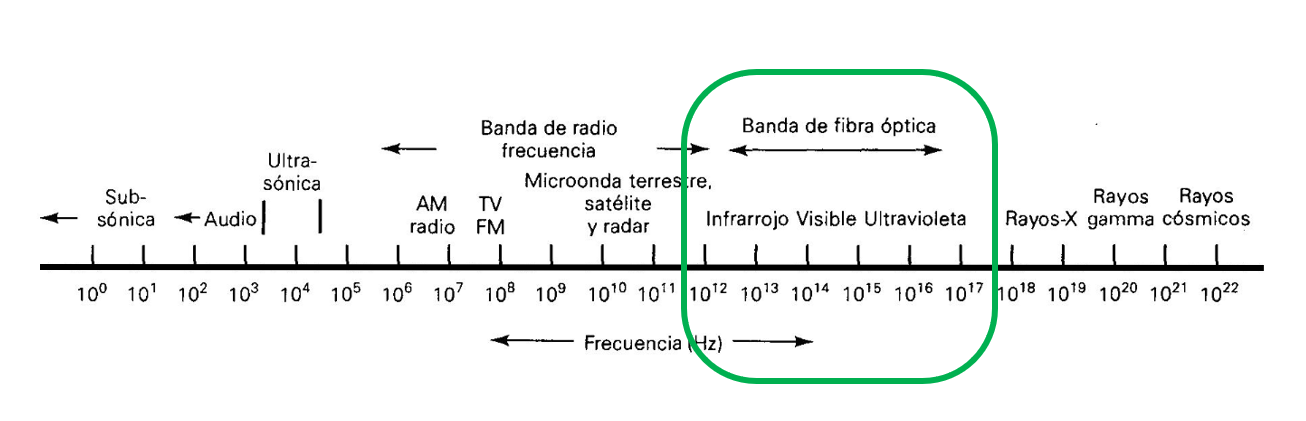
\includegraphics[width=0.95\textwidth]{./img/espectrooptico}
		\caption{Espectro electromagnético en frecuencia.}
		\label{fig:espectroOptico}
	\end{figure}
	
	%--Ventanas de comunicación por FO
	Cabe destacar que dentro del espectro óptico las longitudes de onda habituales para comunicación en fibra óptica están entre los 700nm y 1600nm. Estas se dividen en rangos con mejores características para la transmisión, denominadas ventanas de comunicación. Como se muestra en la figura \ref{fig:ventanaOptica}, son tres las ventanas más utilizadas,\cite{ventanasFO}:
 	\begin{table}[H]
		%\centering
		\hspace{2cm}
		\renewcommand{\arraystretch}{2}
		\begin{tabular}{rrl}
			\textbf{1ª ventana}& 800 a  900 nm  & $\longmapsto$ $\,$ longitud de onda utilizada = 850nm  \\
			\textbf{2ª ventana}& 1250 a 1350 nm & $\longmapsto$ $\,$ longitud de onda utilizada = 1310nm  \\
			\textbf{3ª ventana}& 1500 a 1600 nm & $\longmapsto$ $\,$ longitud de onda utilizada = 1550nm   \\ 
		\end{tabular} 
	\end{table}

	 \begin{figure}[H]
	 	\centering
	 	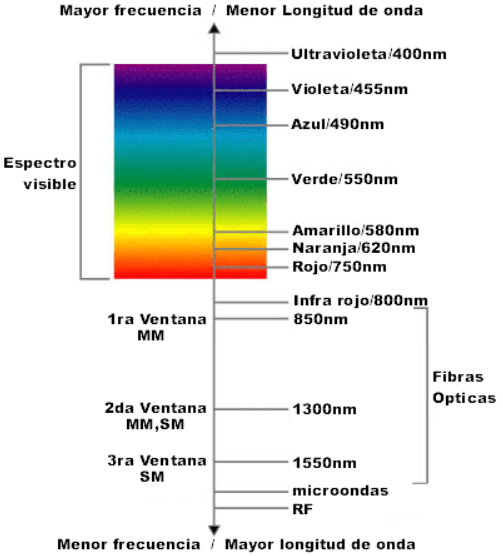
\includegraphics[width=0.5\textwidth]{./img/ventana}
	 	\caption{Longitud de onda fibra óptica junto con el espectro visible. \cite{ventanasFO}}
	 	\label{fig:ventanaOptica}
	 \end{figure}
 	La razón de que las ventanas de comunicación utilizadas se sitúen en las frecuencias indicadas reside en los diferentes comportamientos que tiene la atenuación de las señales en función de la longitud de onda (ver figura \ref{fig:perdidasFrec}). Existen algunas zonas dónde la atenuación es mínima, coincidiendo con la segunda y la tercera ventana. En cambio, en la zona correspondiente a la primera ventana las pérdidas no son mínimas, pero sí que se mantienen constantes. 	
 	
 	\begin{figure}[H]
 		\centering
 		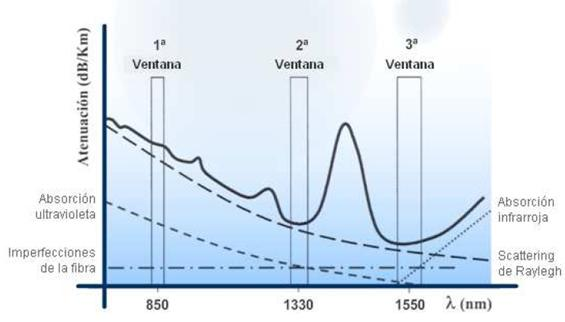
\includegraphics[width=0.8\textwidth]{./img/perdidasFrec}
 		\caption{Atenuación(dB/Km) frente a longitud de onda  $\lambda$ (nm) \cite{imgRadioModo}}
 		\label{fig:perdidasFrec}
 	\end{figure}

 %-- Características físicas de la fibra
 En cuanto a las propiedades físicas de la fibra óptica, son bastante delicadas ya que su grosor no supera por mucho al diámetro del cabello humano y se obtiene de la extrusión del sílice, SiO\textsubscript{2} , es decir, se trata de un filamento de vidrio muy fino. Es por ello que es la fibra óptica estándar está rodeada de una cubierta protectora. 
 
  \begin{figure}[H]
  	\centering
  	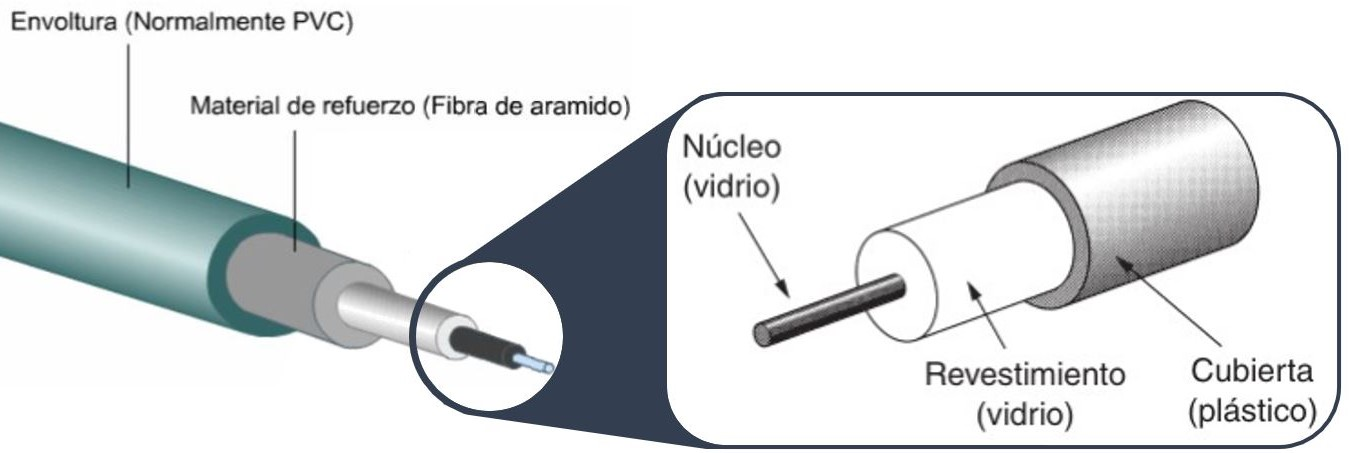
\includegraphics[width=0.87\textwidth]{./img/capas-fibra2}
  	\caption{Capas fibra óptica \cite{imgNucleoFibra,imgCapasFO}} 
  	\label{fig:capasFibra}
  \end{figure} 
  
  
  
 La fibra óptica estándar cuenta varias capas (figura \ref{fig:capasFibra}): núcleo, revestimiento y cubierta (o buffer).  Si la aplicación lo permite, conviene proteger la fibra con más capas externas. En la imagen anterior la fibra está además protegida por un material de refuerzo (fibra de aramido) y una envoltura (PVC).
 
 Tanto el núcleo cómo el revestimiento forman el medio por el cual se propaga la luz. Estas dos capas son tan finas que forman un filamento flexible, pero muy delicado, puesto que es muy propenso a romperse ante dobleces u otras manipulaciones externas. Por ello el resto de las capas son tambien importantes por proporcionar a la fibra protección y haciendo posible su utilización es escenarios de despliegue.
 
 %-- Fabricación FO
 La fabricación de la fibra óptica es un proceso de alta tecnología. Es importante mantener la pureza y la regularidad del núcleo. Esto es complejo, puesto que estamos hablando en algunos casos de núcleos de un grosor entorno a las 8 micras (en fibras monomodo). El grosor estándar de la fibra es de 125 micras(una micra equivale a una millonésima parte de un metro). Para conseguir este resultado el proceso de fabricación consiste en reproducir a escala macroscópica la estructura de la fibra que se quiere obtener. Esta reproducción a gran escala de la fibra deseada se le denomina preforma. Una vez se tiene la preforma, esta se va fundiendo y estirando hasta alcanzar el filamento del diámetro deseado. De una preforma se pueden sacar kilómetros de fibra. Para fabricar la preforma se parte de una barra de vidrio hueca (el vidrio que formará el recubrimiento) y se baña en un gas que contiene unas partículas (lo que formará el núcleo). Al calentar a mil grados, las partículas comienzan a fundirse hasta que el tubo colapsa y forma una vara maciza, que es la preforma. Para fundirla y estirarla esta se coloca verticalmente y se calienta. La complejidad de esta fase reside en mantener constante el flujo y el diámetro del hilo resultante. Además durante esta fase se aprovecha para crear una capa protectora sobre el vidrio (cubierta en la figura \ref{fig:capasFibra}). Finalmente los kilómetros de fibra óptica se enrollan en grandes bobinas. \cite{fabricacionFO}
 
 %-- Fibra Monomodo y multimodo
  \begin{figure}[H]
 	\centering
 	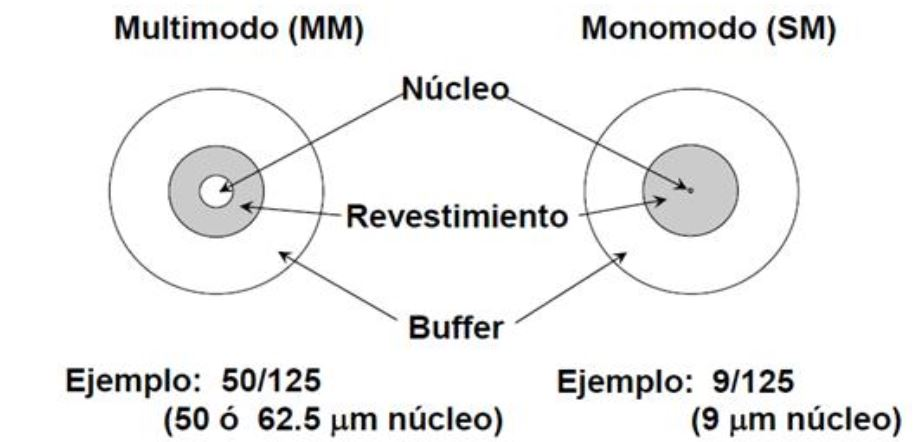
\includegraphics[width=0.6\textwidth]{./img/MM-SM}
 	\caption{Relación grosor fibra multimodo (MM) y monomodo (SM) \cite{imgRadioModo} } 
 	\label{fig:modoMonoMulti}
 \end{figure} 
 
  Dependiendo de la relación de diámetro entre el núcleo y el revestimiento, la fibra fibra será monomodo o multimodo (figura \ref{fig:modoMonoMulti}). Esta diferencia afecta a la propagación de la luz dentro de la guía de onda (figuras \ref{fig:guiaMM}, \ref{fig:guiaSM}, \ref{fig:indiceMultimodo}). Ya se ha comentado que el diámetro de la fibra es de aproximadamente 125 micras. En el caso de las fibras monomodo, el núcleo de estas tiene un diámetro tan pequeño (en torno a 8 micras) que la luz solo puede propagarse en un sólo modo (rayo). Sin embargo, en el caso de las fibras multimodo, al poseer un núcleo mayor (entre 50 o 62.5 micras) soportan la transmisión el múltiples modos, es decir, los rayos de luz viajan en muchas direcciones a través de este. \cite{FOA} 
   
   	\begin{figure}[H]
		\centering
		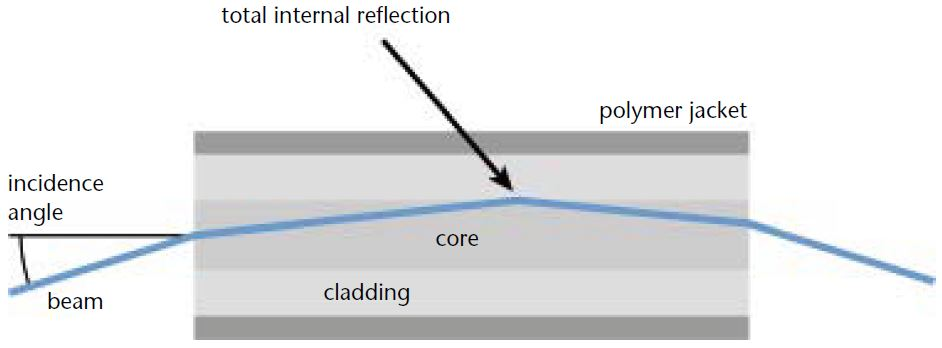
\includegraphics[width=0.7\textwidth]{./img/guiaMM}
		\caption{Corte transversal fibra multimodo en transmisión de luz. \cite{imgMonoMulti} } 
		\label{fig:guiaMM}
	\end{figure} 
  	\begin{figure}[H]
		\centering
		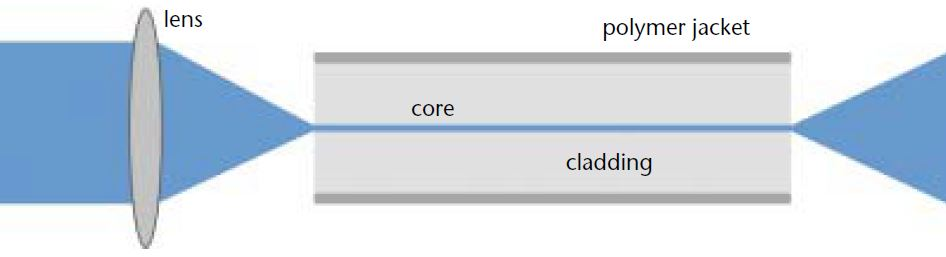
\includegraphics[width=0.7\textwidth]{./img/guiaSM}
		\caption{Corte transversal fibra monomodo en transmisión de luz. \cite{imgMonoMulti} } 
		\label{fig:guiaSM}
	\end{figure}  
 	
 	%-- Relación monomodo y multimodo con las longitudes de onda
 	Relacionando los tipos de fibras ópticas con las ventanas en las que trabajan, las fibras multimodo suelen trabajar en primera y segunda ventana, mientras que las fibras monomodo en segunda y tercera. 

	  	\begin{figure}[H]
		\centering
		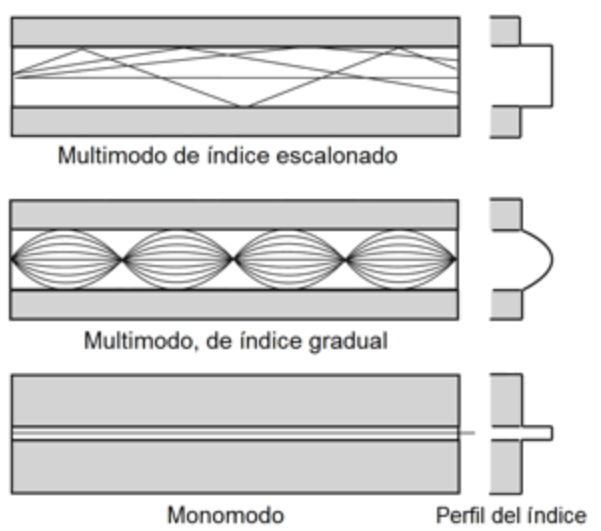
\includegraphics[width=0.5\textwidth]{./img/transFO-esc-grad}
		\caption{Disposición rayos. Multimodo (indice escalonado y gradual) y monomodo. \cite{FOA} } 
		\label{fig:indiceMultimodo}
		\end{figure}
	
 	%-- Otros tipos de FO
 	Además existen otros tipos de fibras menos comunes: la fibra de plástico (POF) y la fibra de sílice con revestimiento de plástico (HCS/PCS). La primera tiene un núcleo de gran diámetro ($1mm$ aproximadamente), puede utilizarse para redes de distancia corta y de baja velocidad. Las fibras de sílice con revestimiento de plástico tienen un núcleo más pequeño ($200\mu m$ aproximadamente) que las fibras de plástico. Estos dos últimos tipos de fibra multimodo generalmente son de índice escalonado, mientras que el resto de fibras multimodo suelen ser de índice gradual. En la figura \ref{fig:indiceMultimodo} se observa como es la diferencia en la distribución de los rayos en un caso y en el otro. En cuanto al tamaño de las fibras, la figura \ref{fig:otrosTiposFO} se representan las diferentes relaciones de tamaños entre los cinco tipos de fibra vistos. \cite{FOA}
 	 	
 	 \begin{figure}[H]
 	 	\centering
 	 	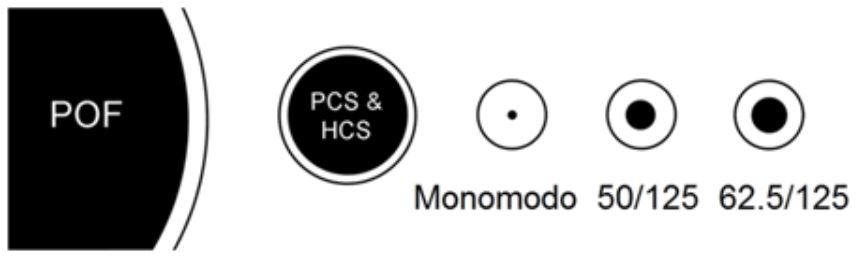
\includegraphics[width=0.7\textwidth]{./img/tiposFO}
 	 	\caption{Relación tamaños fibras ópticas. \cite{FOA} } 
 	 	\label{fig:otrosTiposFO}
 	 \end{figure} 	
  	
 %-- PROPAGACIÓN DE LA LUZ	
 %-- Diferenci de indices de refracción
 La diferencia de índices de refracción entre las capas centrales de la fibra son las que permiten la propagación de la luz a través de esta. El núcleo tiene un mayor indice de refracción que el revestimiento, lo que genera que los rayos de luz se curven a medida que pasan del núcleo al revestimiento, generando una "reflexión interna total" en la fibra. La siguiente imagen (figura \ref{fig:TIR}) sirve para explicar claramente este concepto:
 
 \begin{figure}[H]
 	\centering
 	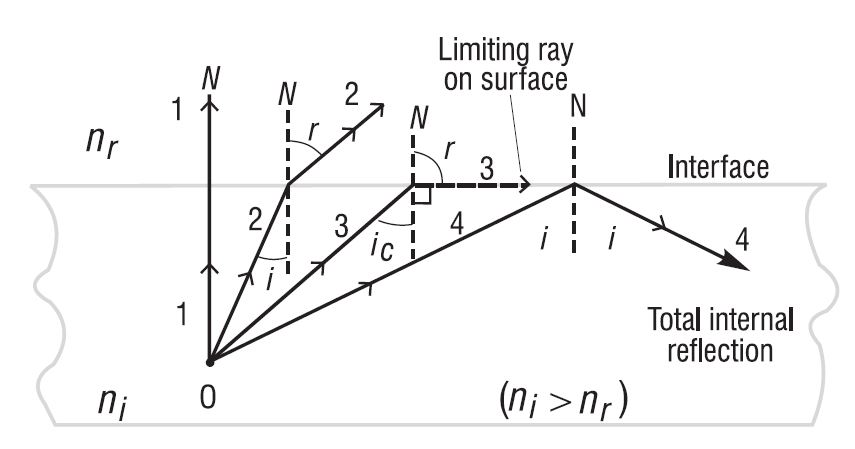
\includegraphics[width=0.66\textwidth]{./img/TIR}
 	\caption{Ángulo crítico y reflexión interna total. \cite{geometriaBasicaFP} } 
 	\label{fig:TIR}
 \end{figure}
 
 %Reflexión interna total
 En la figura \ref{fig:TIR} se ilustran cuatro rayos que se originan en el puno 0, lo que sería el núcleo de la fibra óptica (dónde el indice de refracción \textit{n\textsubscript{i}} es mayor). Entre los cuatro rayos varía el ángulo con el que estos inciden sobre el revestimiento (de menor índice de refracción\textit{n\textsubscript{r}}). Se observa cómo en el rayo número 1 incide con $90\,^{\circ}$ (incidencia normal), no habiendo reflexión y siguiendo el rayo en la misma dirección. En el rayo número 2 incide con un ángulo \textit{i}, y se refracta con \textit{r}. El rayo número 3 incide con el ángulo crítico \textit{i\textsubscript{c}}, suficientemente grande para que el rayo reflejado se propague a lo largo de la interfaz entre los dos medios, quedando atrapado. Por último, el rayo número 4 incide con un ángulo \textit{i} superior al ángulo crítico (ecuación \ref{eq:angCritico}), \textit{i\textsubscript{c}}, consiguiendo que se refleje totalmente en el mismo medio del que incide. Este rayo obedece a la ley de reflexión, siendo su ángulo de reflexión exactamente igual a su ángulo de incidencia. Este fenómeno se denomina \textit{"Reflexión interna total"}, necesario para que suceda la transmisión de señales lumínicas en la fibra óptica. 

	\begin{equation}
		\label{eq:angCritico}
		\hat{i}\textsubscript{c} =  \sin^{-1}\left(\dfrac{n\textsubscript{r}}{n\textsubscript{i}}\right)
	\end{equation}

 La reflexión interna total atrapa la luz hasta cierto ángulo en el núcleo, definiendo la apertura numérica a la que hay que asegurarse de penetrar la luz para que se de el fenómeno de reflexión interna total. Así se fuerza a que la mayoría de los rayos de luz incidan sobre el interfaz y se reflejen, permitiendo la transmisión de la señal lumínica. 
 
 
 \textcolor{rositaoscuro}{//----------------------------------------------------------------------- }\\ 
 %No vamos a hablar más de multimodo
 \textcolor{teal}{(\\Puesto que en la solución llevada a cabo en este trabajo se utilizan fibras monomodo no se va a extender el texto en explicar más conceptos sobre la transmisión en fibras multimodo.\\)\\
 \textcolor{rositaoscuro}{-------------------------------------------------------------------------//}\\}
 
 
 %Sistemas de propagación
   \begin{figure}[H]
 	\centering
 	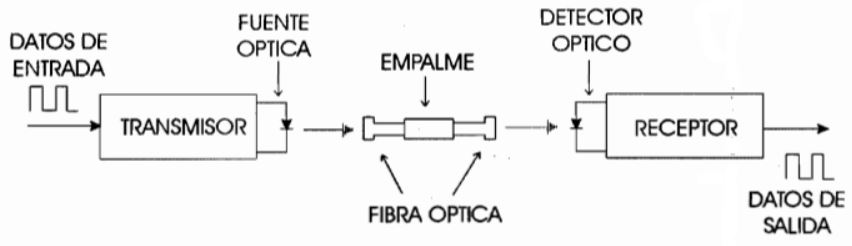
\includegraphics[width=1\textwidth]{./img/TxFOp2p}
 	\caption{Transmisión punto a punto de señales a través de fibra óptica. \cite{txFO} } 
 	\label{fig:TxFOp2p}
 \end{figure} 
 
 Los sistemas de propagación de señales luminosas a través de la fibra óptica componen un medio de transmisión de datos rápido y fiable. En la figura \ref{fig:TxFOp2p} se plasma el procedimiento que sigue la transmisión de datos en un sistema óptico y los elementos que lo componen. Previa a la propagación a través de un medio óptico de una señal eléctrica (analógica o digital) es necesario realizar una conversión de esta a señal óptica. Esto genera una señal óptica a partir de una señal eléctrica en el emisor o fuente de luz situado en el extremo inicial de la comunicación. Realizada la conversión, la señal es transmitida a lo largo de la fibra óptica. Según las características del escenario puede haber una o varias uniones entre fibras a lo largo del canal. Estás pueden realizarse empalmando o utilizando conectores. Una vez la señal óptica atraviesa todo el canal, llega al detector, dónde sucede el proceso inverso al ocurrido en el emisor y a la salida del sistema completo se tiene la señal eléctrica. Esta corresponde a la señal introducida al sistema con una pequeña posibilidad de haber sufrido pérdidas o atenuación debido a la impureza de la fibra, la distancia, las conexiones entre elementos del sistema o cualquier otro evento ajeno al este. Estas modificaciones de la señal de entrada pueden ser contrarrestadas o solventadas en recepción sin suponer un impedimento a una comunicación exitosa.    
  
 Veamos por separado los elementos dibujados en la figura \ref{fig:TxFOp2p}:
 	\begin{itemize}
 	%-Emisores (Transmisión)
 		\item \textit{\textbf{Emisores (Transmisión)}}	
 		% \hspace{0.2cm} 
 		Los emisores de luz forman un papel imprescindible en la transmisión de señales a través de la fibra óptica. Se encargan de convertir la señal eléctrica a señal luminosa, para que esta se pueda propagar por el canal óptico según lo esperado. Principalmente hay dos tipos de fuentes de luz: diodos LED o diodos láser. Dentro de los de tipo láser se distinguen otros tres tipos: láser fabry-perot (\textit{FP}), láser de retroalimentación distribuida (\textit{(DFB)}) y láser de cavidad vertical y emisión superficial (\textit{VCSEL}). Unas de las condiciones más importantes que deben cumplir las fuentes de luz son que operen en la longitud de onda adecuada, se puedan de modular lo suficientemente rápido para transmitir datos y poder acoplarse de forma eficiente a la fibra. \cite{TransRecepFO}
 		
 		 \begin{figure}[H]
 			\centering
 			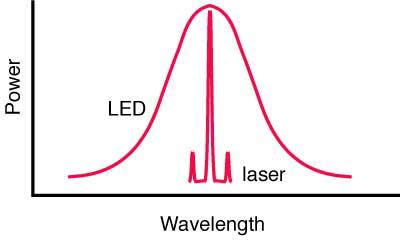
\includegraphics[width=0.35\textwidth]{./img/led-laser}
 			\caption{Relación entre potencia y longitud de onda diodo LED frente a diodo láser. \cite{FOA} } 
 			\label{fig:ledVsLaser}
 		\end{figure} 
 	 	\begin{figure}[H]
 			\centering
 			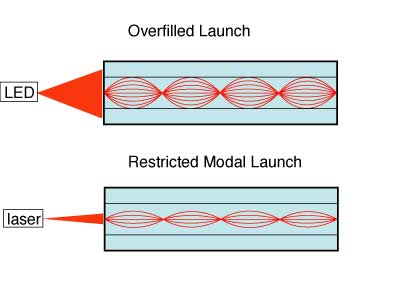
\includegraphics[width=0.55\textwidth]{./img/led-laserEMISION}
 			\caption{Corte transversal de fibra con emisión desde diodo LED frente a diodo láser. \cite{FOA} } 
 			\label{fig:corteledVsLaser}
 		\end{figure} 
 		
 		\begin{itemize}
 			\item \textbf{LED} - \textit{Light Emitting Diodes}\\
 			Consiste en una fuente de luz incoherente. Es una fuente de luz de mayor ancho de banda de operación que en el caso de los diodos láser (véase figura \ref{fig:ledVsLaser} y \ref{fig:corteledVsLaser}). Tiene un espectro de emisión entre los 30-100 nm. En función del material semiconductor con el que se fabrique se pueden emitir desde luz ultravioleta hasta infrarrojos. Para conseguir emitir en un espectro reducido, es necesario polarizarlo y hacerle circular corriente eléctrica. Pueden ser modulados sin dificultad hasta velocidades de 100-200 Mb/s y en algunos casos hasta velocidades de 1 Gb/s. 
 			
 			Además, tienen un comportamiento simple, de fácil fabricación y tienen un coste bajo en comparación a otras fuentes. Su circuitería de alimentación y control es muy sencilla, debido a los bajos niveles de corriente que son necesarios para que funcione el dispositivo y a su relativa inmunidad frente a variaciones de la temperatura. Necesitan baja potencia de alimentación. Su geometría y patrón de radiación es de alta divergencia, el acoplo de luz a la fibra óptica monomodo es difícil, especialmente en los LED de emisión superficial. Son dispositivos fiables, ya que no sufren la degradación de tipo catastrófico y son menos sensibles que los diodos láser a la degradación por envejecimiento. \\
 			
 					\textcolor{rositaoscuro}{//-Resumen: Los LED se basan en emisión espontánea. Por sus características (baja coherencia, divergencia alta, baja potencia óptica de salida, circuitos electrónicos sencillos,...) se emplean habitualmente en combinación con fibras multimodo para enlaces de distancias cortas y velocidades bajas.}
 			
 			\item \textbf{Láser} - \textit{Light Amplification by Stimulated Emission of Radiation}\\
 			Consiste en un tipo de fuente de luz coherente. Tienen mayor capacidad de transmisión de luz, concentran la luz en forma de haces estrechos pero potentes, es decir, emiten de manera direccional e intensa. Es por ello que se suele advertir que mirar con los ojos directamente a este tipo de emisiones es peligroso para la vista. (Véanse figuras \ref{fig:ledVsLaser} y \ref{fig:corteledVsLaser}). Pueden ser modulados en frecuencia y a gran velocidad. Su geometría y patrón de radiación es de relativamente baja divergencia, el acoplo de luz a la fibra óptica monomodo es bastante eficiente. Su composición es más compleja que la del diodo LED. Para conseguir dicha directividad y potencia, internamente la fuente tiene cavidades que combinan medio activo y espejos. Por ejemplo, necesita tener un circuito de realimentación para su control, debido a que se ve afectado por las variaciones de temperaturay a las reflexiones que pueda provocar la potencia óptica incidente en su salida. Debido a ello, son complejos y costosos de fabricar. 
 			
 					\textcolor{rositaoscuro}{//- Resumen Los láseres se basan en emisión estimulada, conseguida formando cavidades que combinan medio activo y espejos para la realimentación. Son de mayores prestaciones que los LED (mayor coherencia, más directivos, mayor potencia de salida,...), pero más complejos y caros. Se pueden usar en fibras monomodo. Los hay de dos tipos, básicamente:\\
 					--Láseres multimodo (Fabry-Perot) que se usan en enlaces de velocidades medias/bajas para distancias medias/cortas\\
 					-- Láseres monomodo (DFB,DBR) que se usan en enlaces de alta capacidad –alta velocidad, distancias largas- y en sistemas WDM}
 			
 			
 		\end{itemize}
  		
  		La tabla \ref{tabla:caractFuentes} compara las características de las diferentes fuentes mencionadas, permitiendo ver también las diferencias entre los diferentes tipos de diodos láser citados.
  		
  		
  		\begin{table}[H]
  			\begin{tabular}{l|c|c|c|c|}
  				\cline{2-5}
  				& \cellcolor[HTML]{EFEFEF}\textbf{LED} & \cellcolor[HTML]{EFEFEF}\textbf{LD F-P} & \cellcolor[HTML]{EFEFEF}\textbf{LD\_DFB} & \cellcolor[HTML]{EFEFEF}\textbf{VCSEL} \\ \hline
  				\multicolumn{1}{|l|}{\cellcolor[HTML]{EFEFEF}Espectro emisión}                 & Ancho                                & Medio                                   & \multicolumn{2}{c|}{Estrecho}                                                     \\ \hline
  				\multicolumn{1}{|l|}{\cellcolor[HTML]{EFEFEF}Directividad}                     & Muy divergente                       & \multicolumn{3}{c|}{Directivo}                                                                                              \\ \hline
  				\multicolumn{1}{|l|}{\cellcolor[HTML]{EFEFEF}Potencia}                         & Baja                                 & \multicolumn{3}{c|}{Alta}                                                                                                   \\ \hline
  				\multicolumn{1}{|l|}{\cellcolor[HTML]{EFEFEF}Velocidad / BW modulación}        & Varios cientos de MHz                & \multicolumn{3}{c|}{Varias decenas de GHz}                                                                                  \\ \hline
  				\multicolumn{1}{|l|}{\cellcolor[HTML]{EFEFEF}Acoplo a la fibra}                & MMF                                  & \multicolumn{2}{c|}{SMF}                                                           & MMF                                    \\ \hline
  				\multicolumn{1}{|l|}{\cellcolor[HTML]{EFEFEF}Curva I-P}                        & Sin $I_{umbral}$; baja pendiente          & \multicolumn{3}{c|}{Con $I_{umbral}$; alta pendiente}                                                                            \\ \hline
  				\multicolumn{1}{|l|}{\cellcolor[HTML]{EFEFEF}Dependencia con temperatura}      & Baja                                 & \multicolumn{3}{c|}{Alta}                                                                                                   \\ \hline
  				\multicolumn{1}{|l|}{\cellcolor[HTML]{EFEFEF}Circuitos electrónicos asociados} & Sencillos                            & \multicolumn{3}{c|}{Complejos}                                                                                              \\ \hline
  				\multicolumn{1}{|l|}{\cellcolor[HTML]{EFEFEF}Seguridad para la vista}          & No peligroso                         & \multicolumn{3}{c|}{Potencialmente dañino}                                                                                  \\ \hline
  				\multicolumn{1}{|l|}{\cellcolor[HTML]{EFEFEF}Tiempo vida útil}                 & Alto                                 & \multicolumn{3}{c|}{Medio (suficiente)}                                                                                     \\ \hline
  				\multicolumn{1}{|l|}{\cellcolor[HTML]{EFEFEF}Coste}                            & Bajo                                 & Medio                                   & Alto                                     & Bajo                                   \\ \hline
  				\multicolumn{1}{|l|}{\cellcolor[HTML]{EFEFEF}Ventana operación}                & 1ª, 2ª                               & \multicolumn{2}{c|}{2ª, 3ª}                                                        & 1ª, 2ª                                 \\ \hline
  			\end{tabular}
  		\caption{Tabla características fuentes de ópticas}
  		\label{tabla:caractFuentes}
  		\end{table}
  	
   	%-Detectores (Recepción)		
 		\item \textit{\textbf{Detectores (Recepción)}}
 			
 		En cuanto al proceso de recepción, consiste en que la señal llega al final del canal y se tiene que dar el proceso inverso que en transmisión. Los detectores tienen la función de convertir las señales ópticas a señales eléctricas para recuperar la información. Son diodos semiconductores encargados de polarizar inversamente la polarización realizada en el diodo emisor.  Al igual que pasaba en la transmisión, existe detección coherente o incoherente(detección directa). El componente del receptor que realiza la conversión óptico-eléctrica es el fotodetector. Se distinguen varios tipos, los más comunes son: los fotodidos PIN y los fotodiodos de efecto de avalancha (\textit{APD}). Aunque merece la pena mencionar los fotoespectrómetros, formados por células CCD integradas y una estructurá optica tan precisa que es capaz de detectar la potencia que la luz recibida proporciona en cada longitud de onda. Volviendo a los receptores PIN y APD, además del fotodetector, el detector puede estar compuesto por un pre-amplificador óptico, pero casi siempre tendrá un pre-amplificador eléctrico para amplificar la señal eléctrica obtenida del fotodiodo, de muy baja corriente. El receptor lo podrá formar también (figura \ref{fig:diagRX}) un filtro óptico, para tomar solo en cuenta las frecuencias de interés. Posterior a la pre-amplificación eléctrica, los elementos de procesado de la señal que se incluyan dependerán del si las señales empleadas por el sistema eléctrico son analógicas o digitales.
 		
	 	\begin{figure}[H]
	 		\centering
	 		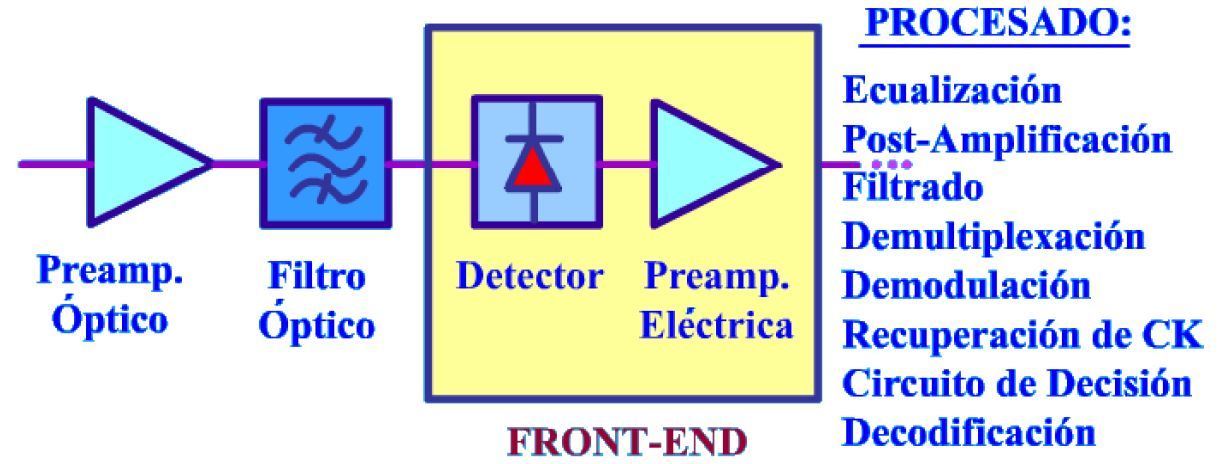
\includegraphics[width=0.65\textwidth]{./img/diagRX}
	 		\caption{Diagrama de bloque receptor} 
	 		\label{fig:diagRX}
	 	\end{figure} 
 	
 		Idealmente los fotodetectores deberián ser altamente sensibles, con alta velocidad de respuesta, poco ruidosos, compactos, robustos y de respuesta lineal. En la práctica es complicado conseguir todos estos atributos en conjunto. Por ejemplo, los APD requieren menor potencia óptica para funcionar que los diodos PIN, pero cuatro veces mayor voltaje de alimentación.
 		
 		\textcolor{rositaoscuro}{//---------------------------------------------------Puedo añadir si eso lo que pone en el siguiente link:}
 		\url{http://www.thefoa.org/tech/ref/appln/transceiver.html}
 	
 	%-Conectores y empalmes
 		\item \textit{\textbf{Conectores y empalmes}}\\

 		Cabe hablar también de los conectores ópticos y empalmes utilizados para unir fibra óptica a fibra óptica u otros elementos del sistema. Teniendo una fibra óptica terminada en algún tipo de conector esta se puede unir a elementos como emisores, receptores, multiplexores y otros elementos, incluso se puede unir a otra fibra terminada en conector con un adaptador macho a macho. Además, para unir dos trozos de fibra es posible realizar una fusión que empalme ambas terminaciones de la fibra. La principal diferencia entre estos dos tipos de uniones es que los conectores unen de manera no permanente, mientras que los empalmes son uniones permanentes. 
 		
 		\begin{figure}[H]
 			\centering
 			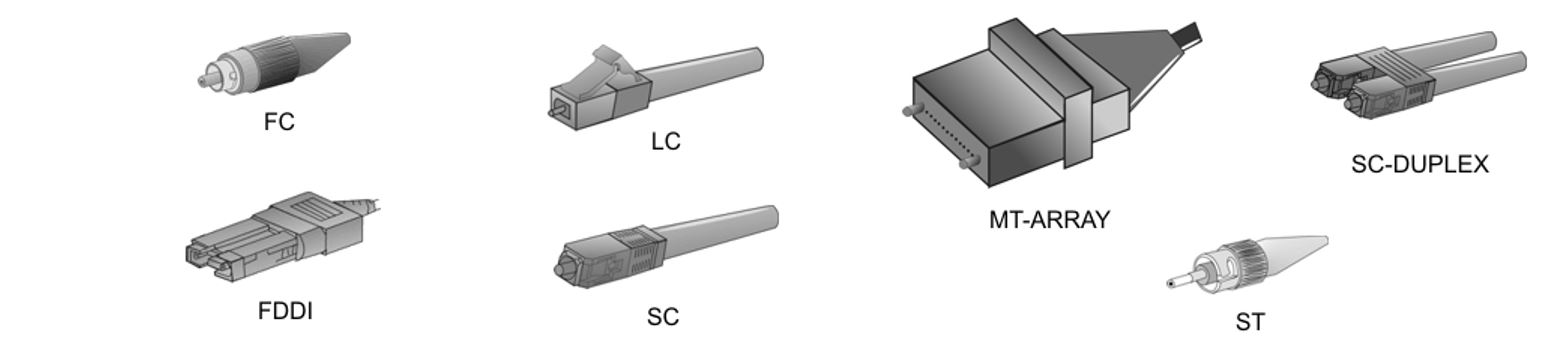
\includegraphics[width=0.95\textwidth]{./img/tiposConect2}
 			\caption{Tipos de conectores de fibra óptica. \cite{TipConectoresFO}} 
 			\label{fig:tiposConect}
 		\end{figure} 
 		
 		Es importante que las uniones no afecten a la calidad de la transmisión, es decir, deben garantizar bajas pérdidas de conectividad. En la figura \ref{fig:tiposConect} se muestra algunos de los conectores más empleados, cada uno de ellos suelen utilizarse en diferentes aplicaciones según sus características. Por ejemplo los utilizados en este trabajo, los conectores FC (\textit{Ferule Connector}) se suelen utiliza tanto en montaje de laboratorio como de campo y sirven en fibras monomodo y multimodo. Además tienen unas pérdidas de inserción IL < 0.34 dB en fibras multimodo y IL < 0.15 dB en fibras monomodo. \cite{TipConectoresFO}\\
 		\begin{figure}[H]
	 		\centering
	 		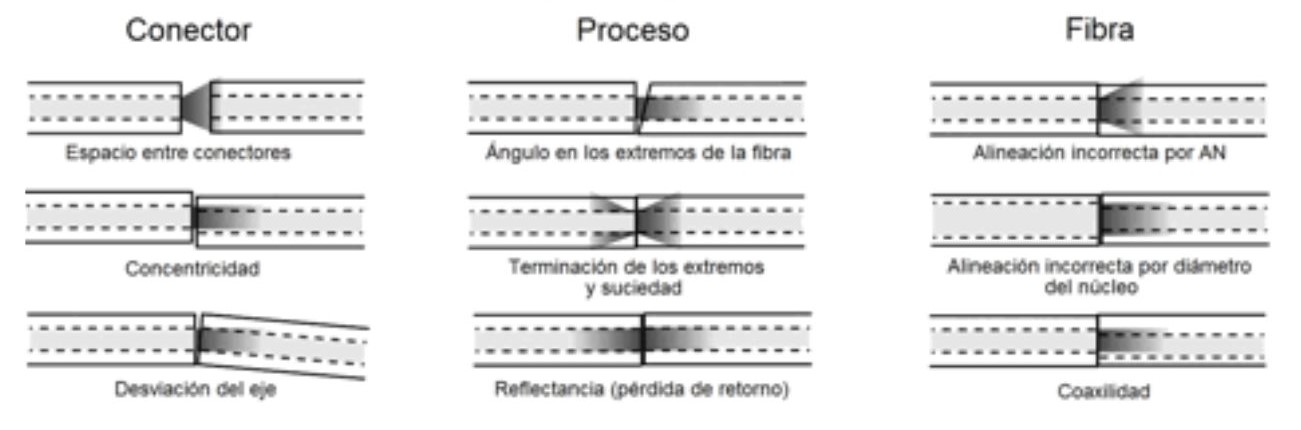
\includegraphics[width=0.85\textwidth]{./img/perdidasOpticas}
	 		\caption{Causas de pérdida óptica en las uniones. \cite{FOAconect}} 
	 		\label{fig:conectLoss}
 		\end{figure}
 		Las pérdidas se pueden reducir cuando los núcleos de las dos fibras son idénticos, están alineados de manera perfecta y se tocan entre sí, los conectores y los empalmes se realizaron adecuadamente y no hay suciedad en la unión. En la figura \ref{fig:conectLoss} se pueden observar diferentes causas de pérdidas en las conexiones de fibra óptica. Además, los conectores pueden tener diferentes formas de férulas (o terminaciones), diferentes tipos de pulidos en el extremo de la fibra donde se realiza la unión (figura \ref{fig:tiposPulidos}), lo que afecta también a las pérdidas resultantes. El extermo de la fibra tiene que estar debidamente limpio y pulido para reducir al máximo ñas pérdidas, ya que una superficie aspera puede dispersar o absorber luz.		
   		\begin{figure}[H]
   			\centering
   			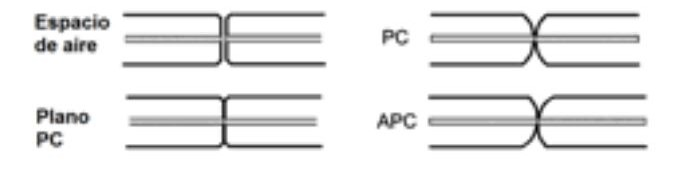
\includegraphics[width=0.55\textwidth]{./img/conectoresPulido}
   			\caption{Tipos de conectores según su pulido. \cite{TipConectoresFO}} 
   			\label{fig:tiposPulidos}
   		\end{figure}

 		En cuanto a los empalmes, que crean una unión permanente entre dos fibras, hay dos tipos: por fusión y mecánicos. En la figura \ref{fig:empalmeTipo} se observa en primer lugar un empalme por fusión y los demás son mecánicos. Los más realizados son los empalmes por fusión por la fiabilidad y la robustez de la unión, así como por brindar pérdidas y reflectancias menores.
 		
 		\begin{figure}[H]
 			\centering
 			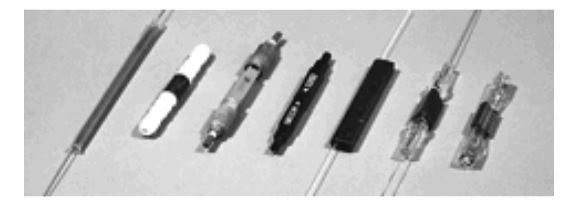
\includegraphics[width=0.5\textwidth]{./img/tiposEmpalme}
 			\caption{Tipos de empalmes. \cite{FOAconect}} 
 			\label{fig:empalmeTipo}
 		\end{figure} 
 	
 		 
 		
 		El proceso de fusión (Figura \ref{fig:procFusion}) consiste en primero pelar, limpiar y cortar los extremos de las fibras que se desee unir. Una vez se dispone en los extremos de la fibra desnuda, cortada con la cortadora de precisión y limpia con un paño adecuado y alcohol, se deben colocar cada una en las guías de la fusionadora. Después se ejecuta el programa de fusión adecuado, según sea la fibra. Por último, se le coloca a la fusión un manguito protector termocontraible o una protección tipo mordaza para que la fusión no se desprenda ante alguna adversidad.
 		
 		\begin{figure}[H]
 			\centering
 			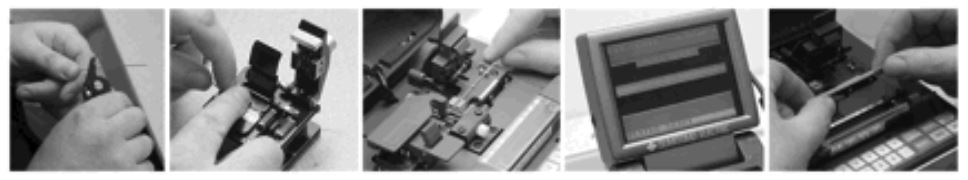
\includegraphics[width=0.85\textwidth]{./img/procesoFusion}
 			\caption{Proceso de empalme por fusión. \cite{FOAconect}} 
 			\label{fig:procFusion}
 		\end{figure}

 	 \end{itemize}					

%-- SENSORES ÓPTICOS	
\subsection{Sensores ópticos} %Tipos de sensores ópticos
\label{sec:sensores3}

		
		Existen en el mercado diversos tipos de sensores ópticos. Estos se pueden clasificar atendiendo a diversos aspectos. A continuación se exponen dos clasificaciones básicas\cite{sensoresOpticos}: 

			\begin{itemize}
				\item[$\cdot$] \underline{En función de la naturaleza del parámetro a cuantificar}
				\begin{itemize}
					\item Sensores químicos: Sirven para detectar variación de cantidad de ciertos componentes químicos. Además en este grupo se incluyen los biosensores.
					\item Sensores físicos: Utilizados para medir parámetros físicos (temperatura, presión, espesor, etc.)
				\end{itemize}
				\item[$\cdot$] \underline{En función de la naturaleza de la propiedad óptica medida}
				\begin{itemize}
					\item Sensores de absorbancia
					\item Sensores de reflectancia
					\item Sensores se luminiscencia (fluorescencia, quimioluminiscencia y bioluminiscencia)
					\item Sensores de dispersión Raman
					\item Sensores de índice de refracción
					\item etc.
				\end{itemize}
				\end{itemize}
			
			
				En este trabajo se van a utilizar sensores de difracción de Bragg, que son sensores que cuantifican parámetros físicos a través de mediciones ópticas del índice de refracción.
		
	\begin{itemize}
		\item \textit{\textbf{Redes de difracción de Bragg \textit{(FBG - Fiber Bragg Grating)}}}	
		
		\begin{figure}[H]
			\centering
			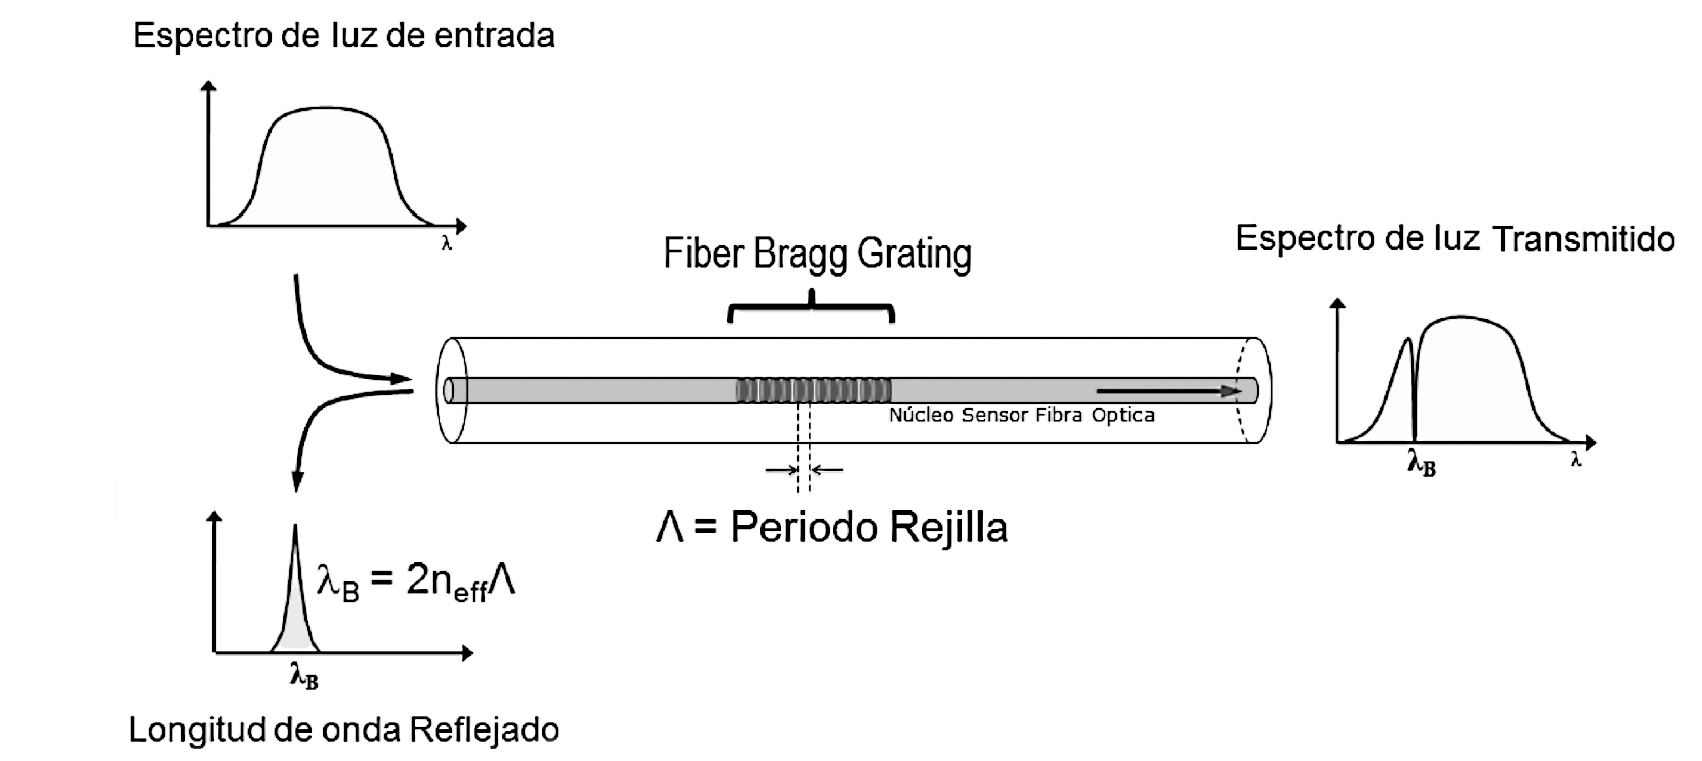
\includegraphics[width=0.85\textwidth]{./img/operacionFBG}
			\caption{Funcionamiento de un sensor de fibra óptica FBG \cite{funcionamientoFBG}} 
			\label{fig:funcionamientoFBG}
		\end{figure}		
		
		Los sensores de fibra óptica basados en redes de difracción de Bragg (\textit{Fibre Brag Gratings}), también denominadas FBGs, están diseñados para reflejar longitudes de onda determinadas (según el diseño) de la luz y transmitir el resto (Figura \ref{fig:funcionamientoFBG}). Para ello se crea en el núcleo de la fibra una variación periódica del índice de refracción, conocido cómo rejilla tipo Bragg. Esta variación sólo afecta a la transmisión de cierta longitud de onda, la que refleja. Este tipo de fenómeno se puede utilizar cómo filtro bloqueador de una longitud de onda, además de para medir parámetros físicos cómo la deformación o la temperatura. Por ejemplo, es muy común su uso para la monitorización de estructuras como puentes \cite{FOSensorFrancis}. 
		
		\begin{figure}[H]
			\centering
			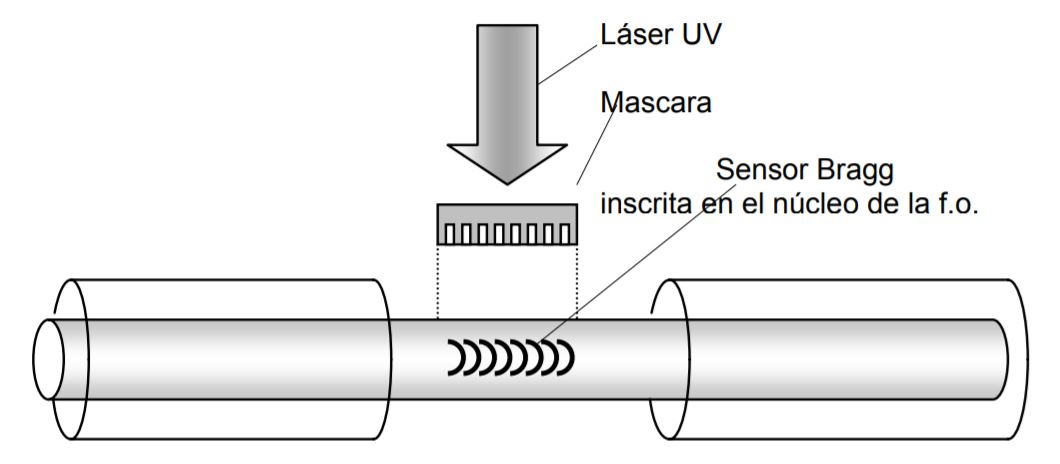
\includegraphics[width=0.75\textwidth]{./img/FBGmanufactur}
			\caption{Proceso de generación del sensor de Bragg en la fibra. \cite{tesisUPMmalte}} 
			\label{fig:manufacturaBragg}
		\end{figure}
		
		 Para conseguir en el núcleo la variación permanente del índice de refracción se utiliza una fuente de luz ultravioleta (UV). De esta manera se inscribe una rejilla tipo Bragg en una fibra monomodo (figura \ref{fig:manufacturaBragg}). Comúnmente se utiliza fibra de sílice dopada con germanio, por su fotosensibilidad (capacidad de cambio del índice de refracción del núcleo con la exposición a la luz UV). En función de la intensidad y la duración de la exposición y de la fotosensibilidad de la fibra se consigue una variación del índice de refracción mayor o menor. 
		
		En resumen, los sensores de fibra de Bragg consisten en una fibra óptica monomodo, dónde, en un segmento reducido de esta, se encuentra una rejilla tipo Bragg. Siendo esta la que genera en el núcleo de la fibra el cambio periódico de índice de refracción \cite{defFBG}.\\
		
		Existe una relación matemática entre la longitud característica de la FBG o longitud de la onda reflejada ($\lambda\textsubscript{B}$), el índice de refracción efectivo ($\eta\textsubscript{eff}$) y el periodo de la red de Bragg ($\Lambda$), como se puede ver en la ecuación \ref{eq:condicBragg}, dónde se define la longittud de la onda reflejada, $\lambda\textsubscript{B}$: 
			\begin{equation}
				\label{eq:condicBragg}
				\lambda=\lambda\textsubscript{B} = 2\eta\textsubscript{eff}\Lambda	
			\end{equation}
				
		A partir de estos conocimientos se deduce cómo funciona la medición de deformaciones. Cuando se genera una deformación de la fibra y cambia la distancia entre las rejillas de Bragg, se genera una variación del índice de refracción al variar el periodo de la red de Bragg. Es decir, al deformarse la FBG se tiene una $\Lambda$ diferente respecto a la de reposo, cuando no se genera ninguna deformación. En el caso de las variaciones de temperatura generan un cambio de índice de refracción del silicio, debido al efecto termoóptico \cite{termoDeformFBG}. 
		
		\begin{figure}[H]
			\centering
			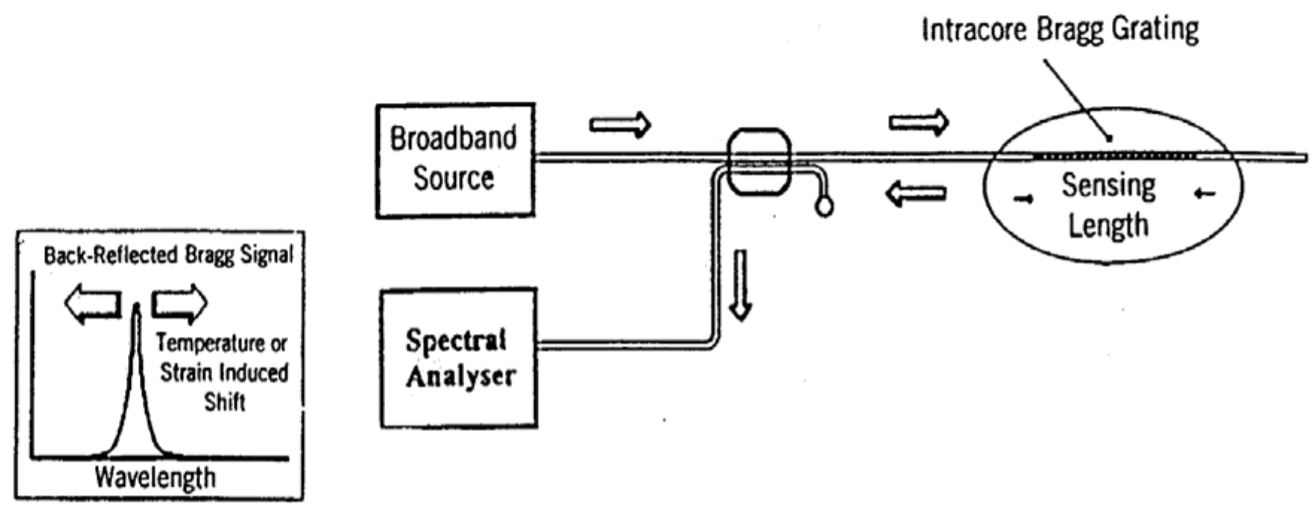
\includegraphics[width=0.85\textwidth]{./img/medicBragg}
			\caption{Representación esquemática de un sistema de  medición de deformaciones mediante fibras ópticas con redes de Bragg y analizador espectral óptico. \cite{tesisUPMmalte}} 
			\label{fig:medicBragg}
		\end{figure}
		
		Para utilizar las FBGs cómo sensores se puede construir una distribución como la de la figura \ref{fig:medicBragg}. En primer lugar, se manda un pulso a través de la fibra, y se pone un analizador de espectros para anotar las variaciones en la longitud de onda de Bragg ($\lambda\textsubscript{B}$). Según sea el escenario a sensar pueden ser necesarias más de una FBG. Para ello se puede realizar una configuración en serie (empalmando FBGs) o en paralelo (utilizando multiplexores). 
		
		\begin{figure}[H]
			\centering
			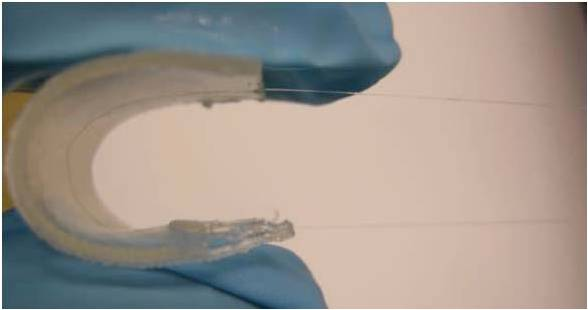
\includegraphics[width=0.65\textwidth]{./img/flexibleFBG}
			\caption{FBG embebida en un material flexible. \cite{nedomaPDMS}} 
			\label{fig:flexibleFBG}
		\end{figure}
	
		Además, para proteger la FBG es conveniente cubrirla con un material flexible (figura \ref{fig:flexibleFBG}), como por ejemplo el policloruro de vinilo (PVC) o el polidimetilsiloxano (PDMS). En este trabajo se utiliza como material protector y estructura del guante el PDMS, expuetso en el siguiente punto.
	
\end{itemize}


%-- POLIDIMETILSILOXANO - PDMS	
\subsection{Polidimetilsiloxano (\textit{PDMS})}
\label{sec:pdms3}
	
	Dentro de la familia de los polímeros orgánicos basados en silicio se encuentra el polidimetilsiloxano, también conocido como PDMS. Otro término por el que se le conoce es dimeticona, un tipo de aceite de silicona. Para abreviar, a partir de este punto en el documento se referirá a él como PDMS. El polidimetilsiloxano es un material cristalino, flexible y fácil de modelar \cite{propPDMS}.
	
	\begin{figure}[H]
		\centering
		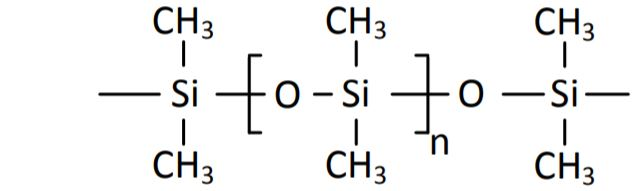
\includegraphics[width=0.45\textwidth]{./img/compPDMS}
		\caption{Composición química del PDMS. \cite{nedomaPDMS}} 
		\label{fig:compFBG}
	\end{figure}
	
	Su formulación química es $(H_{3}C)_{3}SiO[Si(CH_{3})_{2}O]_{n}Si(CH_{3})_{3}$ (figura \ref{fig:compFBG}), siendo $[Si(CH_{3})_{2}O]_{n}$ el monómero presente n veces en la molécula del PDMS según la proporción de este con el agente de curación \cite{propPDMS}.  	
 
 	Para su fabricación se mezcla el monómero con el agente de curación siguiendo una proporción n:1, en función de la consistencia con la que se desee el elastómero resultante. Cuanto mayor sea la n, mayor será la solidez del PDMS. Una vez hecha la mezcla es necesario que esta cure, ya sea a temperatura ambiente o aplicándole calor para que cure más rápidamente.
  
 	\begin{figure}[H]
	 	\centering
	 	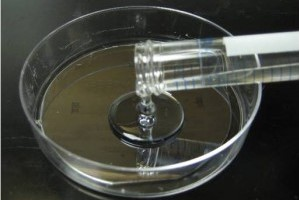
\includegraphics[width=0.49\textwidth]{./img/liquidoPDMS}
	 	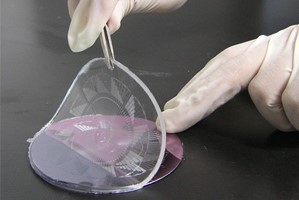
\includegraphics[width=0.49\textwidth]{./img/solidoPDMS} 
	 	\\(a)\hspace{7cm}(b)
	 	\caption{(a) PDMS en estado líquido \cite{liquidoPDMS} (b) PDMS en estado sólido, trás la curación \cite{solidoPDMS}} 
	 	\label{fig:slPDSM}
	 \end{figure}
  \textcolor{teal}{TENGO QUE ELEGIR ENTRE UNA PAREJA DE IMAGENES U OTRA, O UNA DE CADA. Debajo dejo los links de las de abajo por si necesito ponerlos en la bibliografia.\\}
  	\begin{figure}[H]
	 	\centering
	 	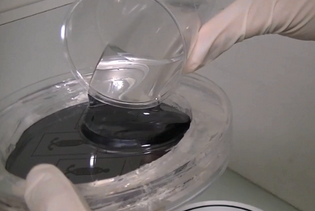
\includegraphics[width=0.49\textwidth]{./img/liquidPDMS}
	 	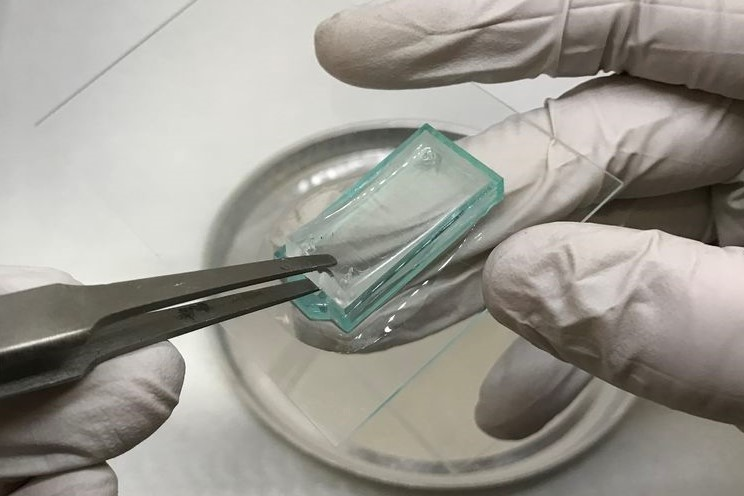
\includegraphics[width=0.49\textwidth]{./img/solidPDMS} 
	 	\\(a)\hspace{7cm}(b)
	 	\caption{(a) PDMS en estado líquido \cite{liquidoPDMS} (b) PDMS en estado sólido, trás la curación \cite{solidoPDMS}} 
	 	\label{fig:slPDSM2}
	 \end{figure}
 
 	\url{https://www.elveflow.com/microfluidic-tutorials/soft-lithography-reviews-and-tutorials/introduction-in-soft-lithography/pdms-softlithography-replication/}
 
	\url{https://www.instructables.com/id/Making-a-PDMS-Microfluidic-Device-With-Maskless-Mo/}
	
  	 La utilización de este elastómero en el ámbito de este trabajo es una buena opción ya que es inofensivo, no tóxico, no inflamable y eléctricamente no conductor.\cite{nedomaPDMS}

	% Material empleado para embeber las FBGs.


		
%-- LABVIEW 	
\subsection{LabVIEW (\textit{\underline{Lab}oratory \underline{V}irtual \underline{I}nstrument \underline{E}ngineering \underline{W}orkbech})}

\label{sec:labview3}



	\begin{figure}[H]
		\centering
		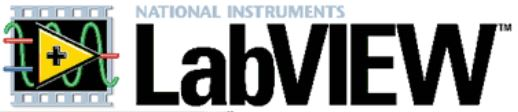
\includegraphics[width=0.45\textwidth]{./img/LabVIEWicon}
		\caption{Logo LabVIEW. }
		\label{fig:LabVIEWicon}
	\end{figure}

	LabVIEW es un software de National Instruments de ingeniería que pretende simplificar el diseño de sistemas software distribuidos de pruebas, medidas y control \cite{LabVIEWpage}. Es un lenguaje y un entorno de programación gráfica desarrollado por National Instruments. 
	
	En sus inicios LabVIEW estaba orientado únicamente a aplicaciones de control de equipos electrónicos utilizados para el desarrollo de sistemas de instrumentación. Tiene dos ventanas principales: el \textbf{Panel frontal} y el \textbf{Diagrama de bloques}, como se ve en la figura \ref{fig:ejLabVIEW}. El panel frontal alberga los botones, pantallas, etc. con el que el usuario interactúa una vez está desarrollado el software, interfaz de usuario. Mientras que el diagrama de bloques corresponde a la circuitería interna del programa, dónde se interconectan los elementos del panel frontal para operar con ellos, dando lugar a la programación del backend del software \cite{LabVIEWbook}. 
	
  	\begin{figure}[H]
		\centering
		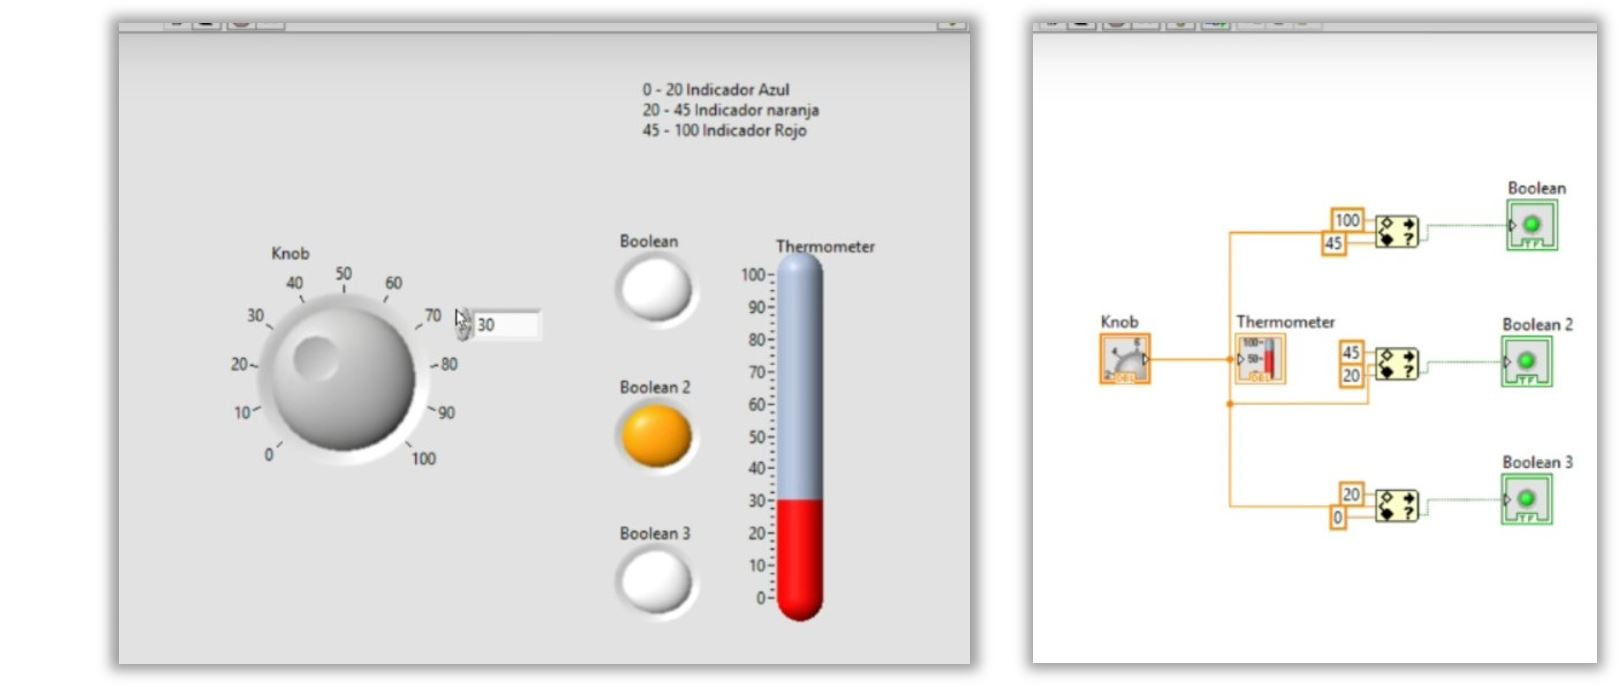
\includegraphics[width=0.95\textwidth]{./img/LabVIEWej}
		\\\hspace{2.5cm}(a)\hspace{6.5cm}(b)
		\caption{(Ejemplo sencillo de LabVIEW: (a) Frontend; (b) Backend}\cite{LabVIEWyt} 
		\label{fig:ejLabVIEW}
	\end{figure}

	En LabVIEW la programación se realiza en el Diagrama de bloques. Los programas están compuestos por los siguientes elementos: controles, funciones e indicadores. Estos elementos se conectan mediante ``cables''. De esta manera se genera el programa, definiendo la ``circulación'' de los datos.  
	

 \textcolor{rositaoscuro}{asdf}
 \textcolor{teal}{sdffsd}
%--Desarrollo del prototipo



\section{Desarrollo del prototipo}
\label{sec:prototipo3}
%[Esta parte de desarrollo del proyecto parte de otro trabajo. Aquí mencionar algo que diga el trabajo de Silvia y mencionarla en la bibliografía.]

La realización del primer desarrollo se origina a partir de un trabajo realizado con anterioridad en el grupo de investigación de la universidad\cite{SilviaTFM}. Se mejora el soporte físico (hardware) y se desarrolla un nuevo programa con un interfaz de usuario simple e intuitivo.
El prototipo consiste en un prototipo técnico y funcional de un guante sensorizado para medir los ángulos de flexión de los nudillos y la muñeca.

 \textcolor{rositaoscuro}{Tengo que sacar una foto mejor que esta donde se vean además el interrogador y la fuente.!!!}
	\begin{figure}[H]
		\centering
		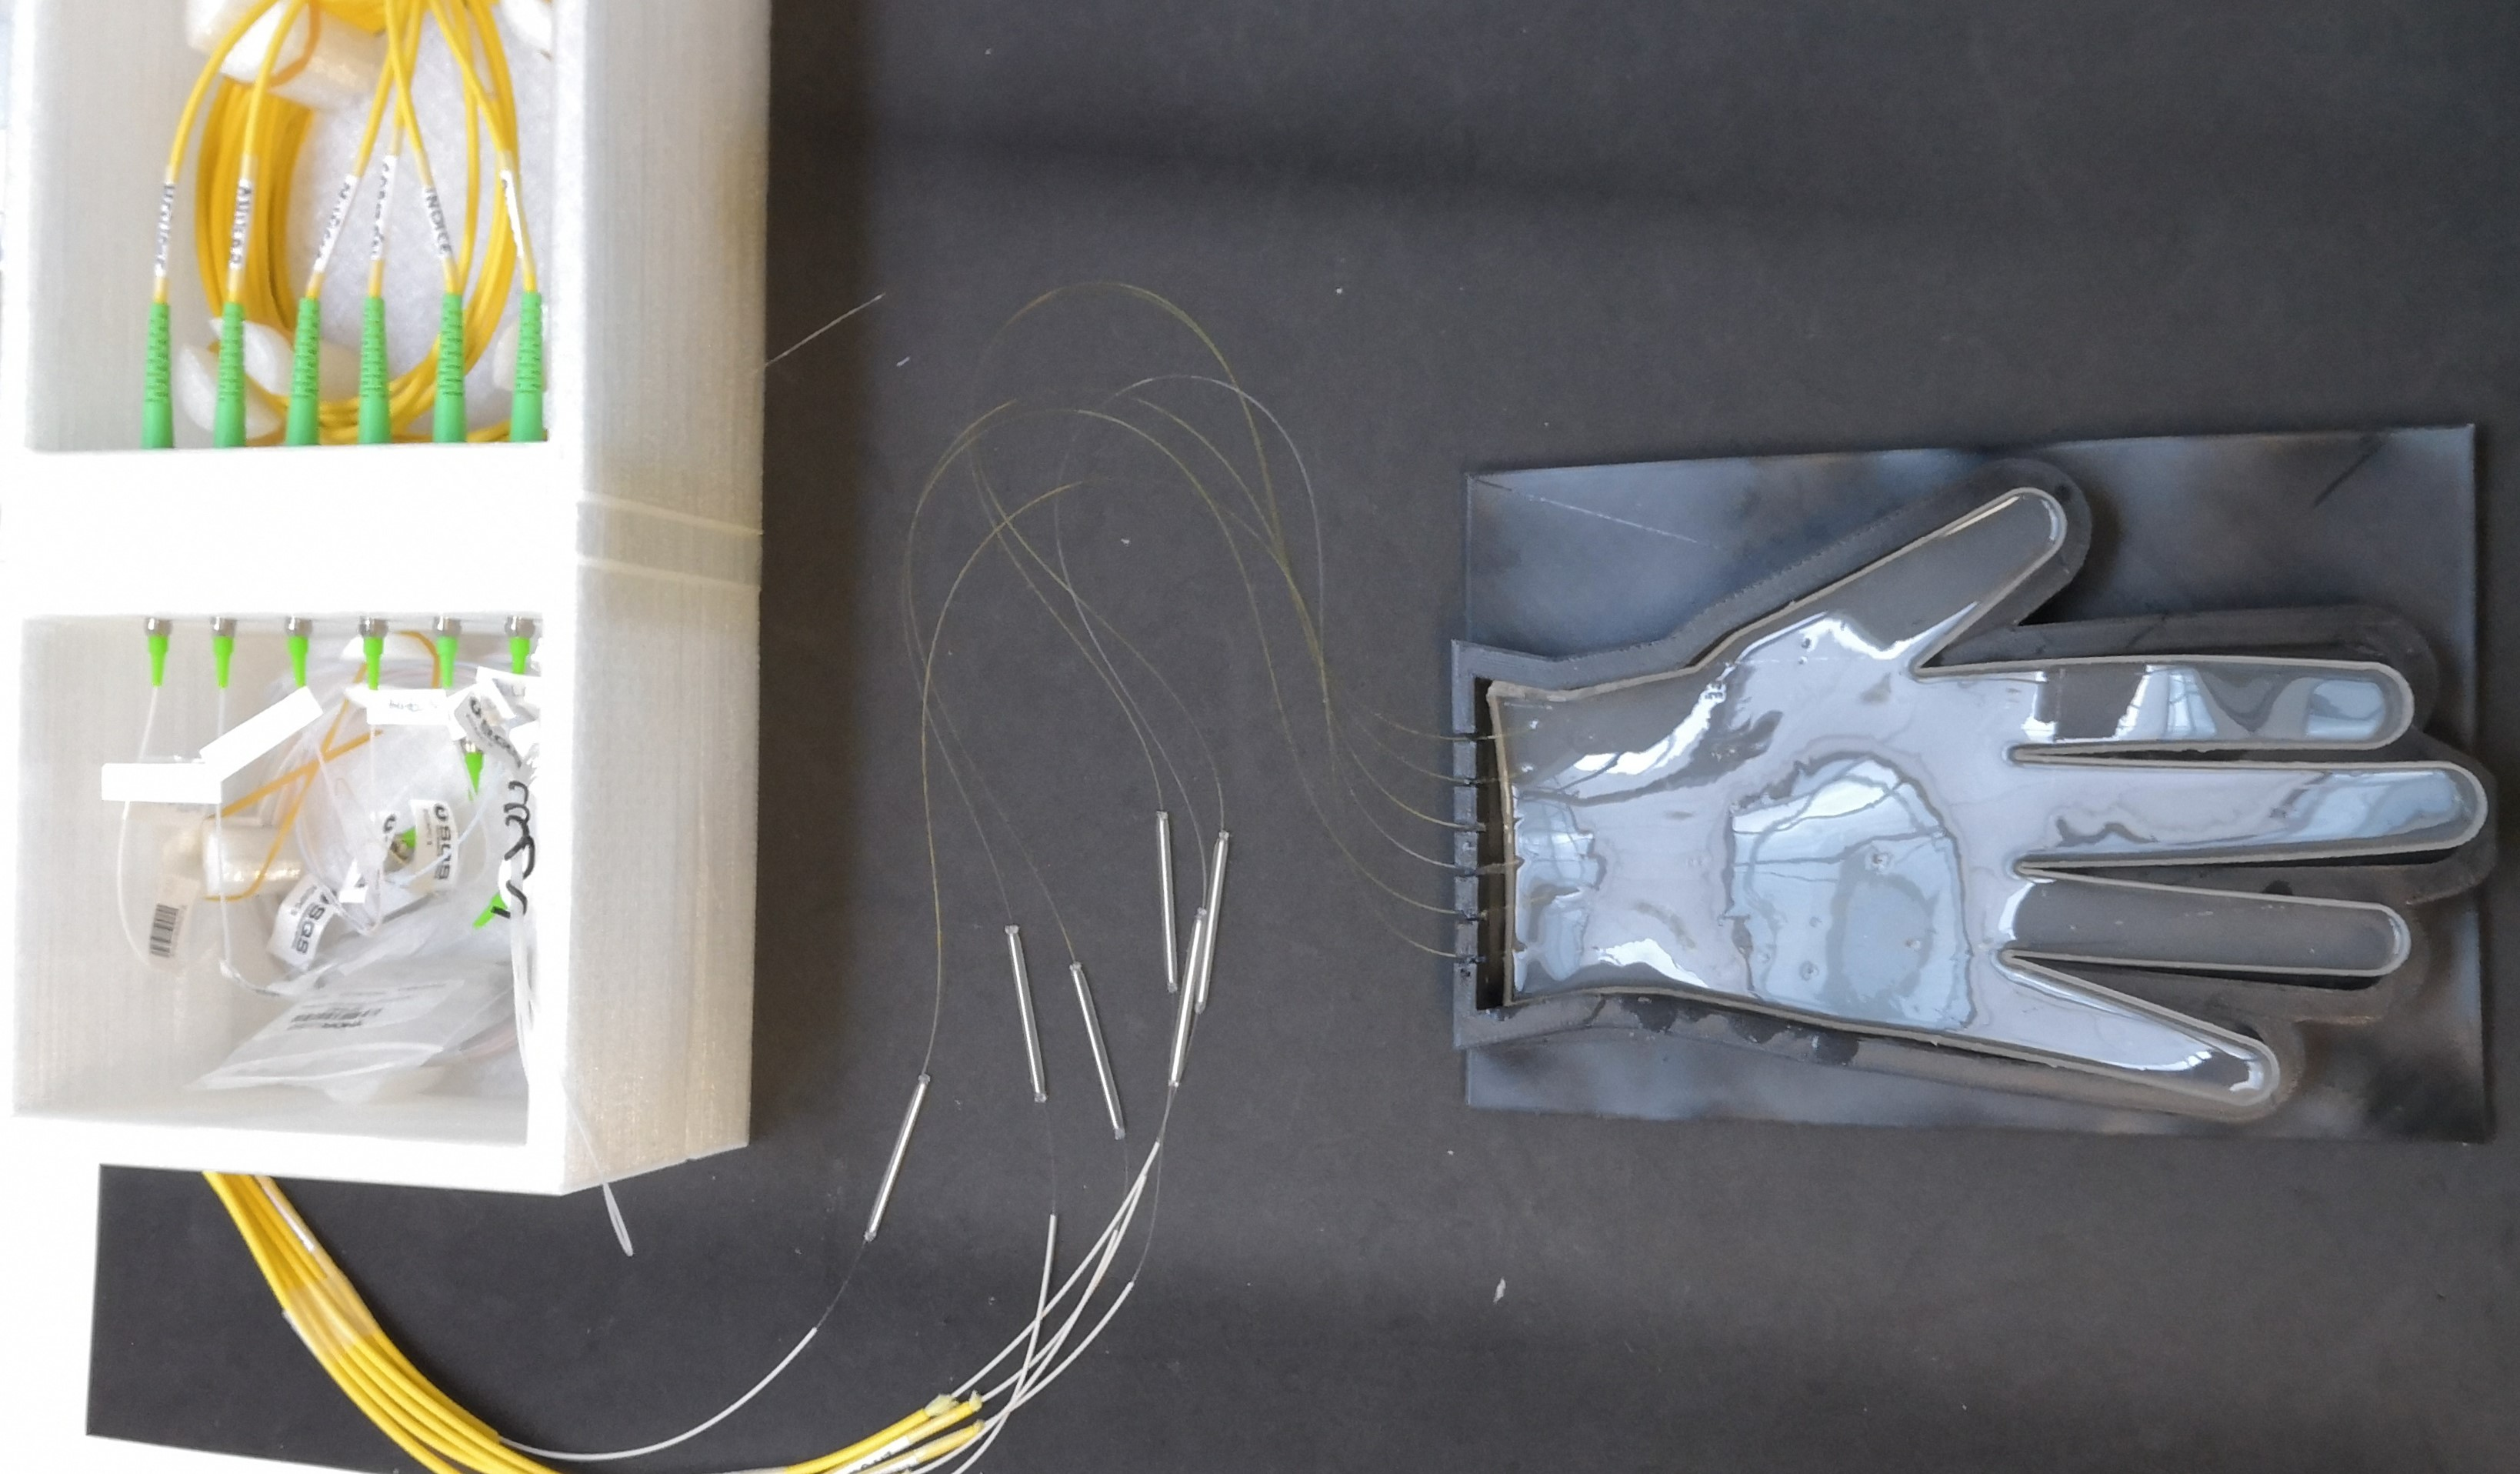
\includegraphics[width=0.85\textwidth]{./img/prototipo}
		\caption{Prototipo con Sensores de fibra FBG.} \label{fig:prototipoFBG}
	\end{figure}


 
\subsection{Materiales}
\label{sec:materiales3}
En este apartado se disponen brevemente los componentes utilizados para el desarrollo del prototipo. 

\begin{figure}[H]
	\centering
	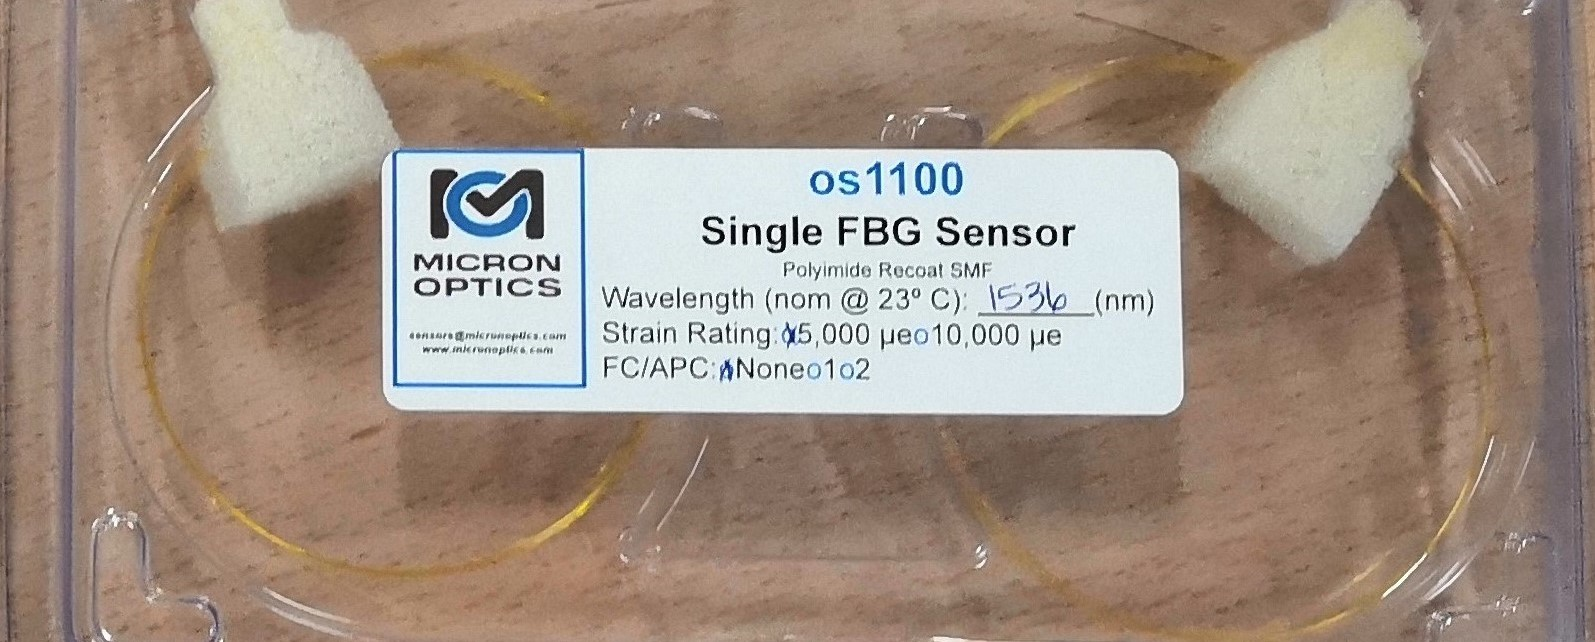
\includegraphics[width=0.60\textwidth]{./img/fibraBraggpaquete2}
	\caption{FBG de longitud de onda de 1536nm en su envoltura de compra.} \label{fig:FBGpaquete}
\end{figure}

Las fibras de rejilla de Bragg (FBG) empleadas son de la empresa Micron Optics (ver figura \ref{fig:FBGpaquete}). Consisten en un FBG centrado en una óptica recubierta don poliimida de dos metros de longitud. Se emplean las siguientes longitudes de onda para cada FBG según la flexión a medir:

\begin{table}[H]
	\centering
	\begin{tabular}[t]{|r|c|}
		\hline
		& Longitud de onda del sensor\\
		\hline
		\hline
		Dedo pulgar & 1532 nm \\
		\hline
		Dedo índice & 1548 nm \\
		\hline
		Dedo corazón & 1576 nm \\
		\hline
		Dedo anular & 1568 nm \\
		\hline
		Dedo meñique & 1560 nm \\
		\hline
		Muñeca & 1541.26 nm \\
		\hline
	\end{tabular}
	\caption{Tabla longitud de cada sensor FBG}
	\label{tabla:mmedidas 80 cm}
\end{table}

Puesto que las fibras de Bragg resultan muy sensibles ante roturas y la aplicación del prototipo precisamente consiste en contorsionar las fibras es necesario embeber las fibras en un material moldeable pero rígido. Para ello se emplea PMDS, cuyas características ya se citan con anterioridad en este documento. En los siguientes apartados se expone con más detalle la fabricación del guante en PDMS. 

El conexionado entre el guante y los demás elementos que componen el prototipo se realiza con cables de fibra óptica monomodo unidos a través de conectores o empalmes. Los empalmes se han realizado mediante fusión con protección termocontraible. Los conectores utilizados para la fibra son los de Férula (\textit{Ferule Connector - FC}).

Para que llegue el pulso transmitido a cada una de las fibras de Bragg hace falta un dispositivo que se capaz de dejar pasar la luz de una sola fibra a varias y combinar en el sentido inverso los pulsos de luz que retornen. Esta función la cumple un divisor de fibra óptica. Se ha empleado un splitter de PLC de una entrada y ocho salidas terminadas en conectores de férula, de las cuales sólo serán necesarias seis (ver figura \ref{fig:splitter}).

\begin{figure}[H]
	\centering
	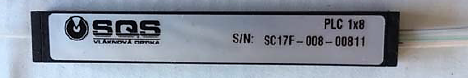
\includegraphics[width=0.75\textwidth]{./img/splitter1a8}
	\caption{Splitter de PLC de 1:8} \label{fig:splitter}
\end{figure}

En cuanto a la transmisión de la luz y su posterior recepción se necesita una fuente y un interrogador. 

La fuente es un emisor de luz de banda ancha que puede provenir de un diodo superluminiscente (SLED) o de emisión espontánea amplificada (ASE).  La fuente integrada en el prototipo es la fuente de diodo superluminiscente (SLED) DL-BP1-1501A de Ibsen Photonics (ver figura \ref{fig:FuenteInterrogador}). Esta fuente es comunmente utilizada para sistemas que utilizan FBGs. Emite pulsos de 70nm de ancho de banda en el rango de los 1550nm. La versión empleada dispone de una interfaz de LabView que permite configurar sus parámetros de emisión cuando fuera necesario. La fuente necesita ser configurada una vez y funciona según su última configuración la próxima vez que se encienda. 

El interrogador es el dispositivo que detecta la señal de luz proveniente de la fibra y, en este escenario, la transmite al ordenador. En este proyecto se trabaja con el interrogador USB I–MON 256/512 del proveedor Ibsen Photonics, al igual que la fuente (ver figura \ref{fig:FuenteInterrogador}). Este interrogador incluye un software implementado en LabView que sirve de herramienta para el usuario para visualizar la detección de luz desde el ordenador a través del puerto USB en tiempo real.  Este software sirve de base para la realización del interfaz de este proyecto. 

\begin{figure}[H]
	\centering
	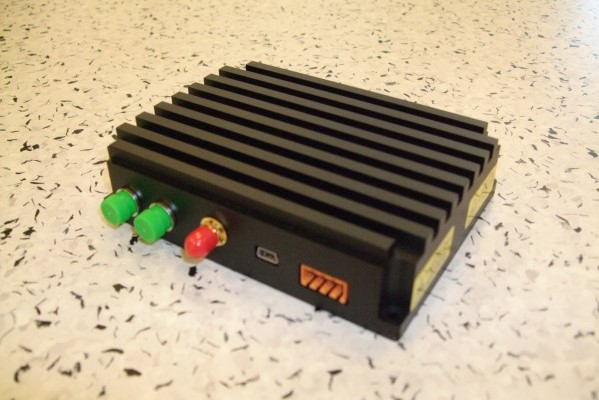
\includegraphics[width=0.49\textwidth]{./img/fuente}
	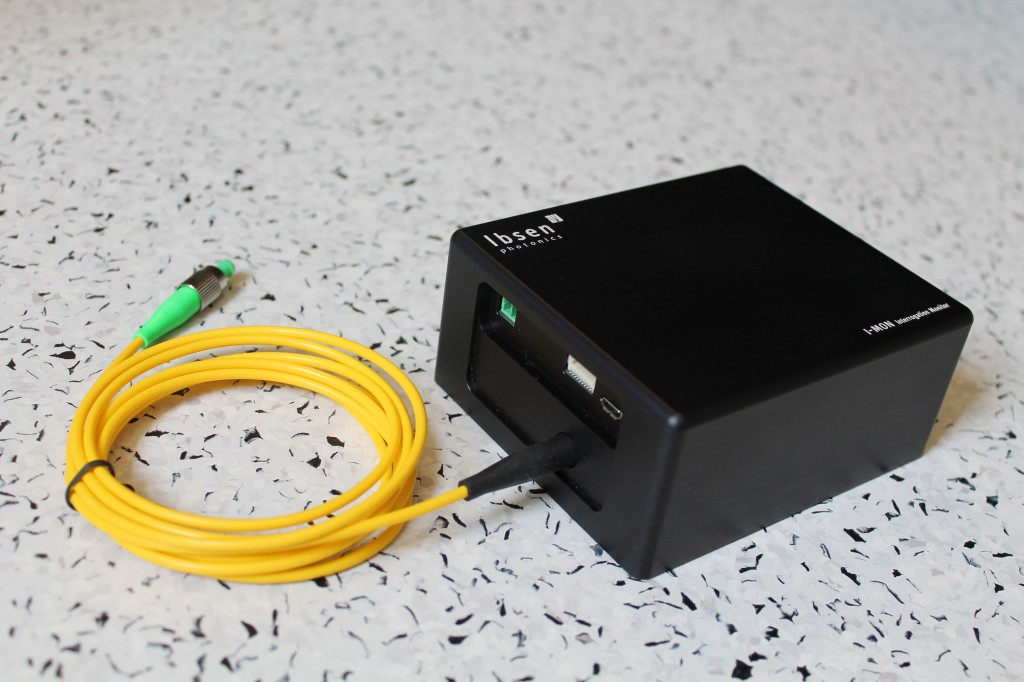
\includegraphics[width=0.49\textwidth]{./img/interrogador} 
	\\(a)\hspace{7cm}(b)
	\caption{(a) Fuente \cite{fuente} (b) Interrogador \cite{interrogador}} 
	\label{fig:FuenteInterrogador}
\end{figure}



Para el desarrollo del software se utiliza un portátil Asus GL502VSK con 32,0 GB de memoria física (RAM) y un procesador Intel(R) Core(TM) i7-7700HQ CPU @ 2.80GHz.  

Además se han diseñado y fabricado el molde para fabricar el molde y  un armazón para almacenar de manera organizada y segura el cableado de las fibras junto con el splitter.

\subsection{Instrumental}
\label{sec:instrumental3}
Este prototipo conlleva el uso de una variada instrumentación. A continuación se mencionan algunos de los instrumentos físicos más notables empleados.  

Para la manufacturación del molde y del armazón se ha empleado tecnología de impresión 3D en material plástico PLA. Se han utilizado dos modelos de impresora debido a la disponibilidad de estas en la universidad, la impresora Hephestos de BQ y Witwox de BQ también (ver figura \ref{fig:impresoras3D}). Son muchos los materiales con los que se pueden realizar impresiones en 3D a partir de un diseño, en este caso se ha escogido el PLA por ser barato y suficiente para las características necesarias en el prototipo.
    
\begin{figure}[H]
	\centering
	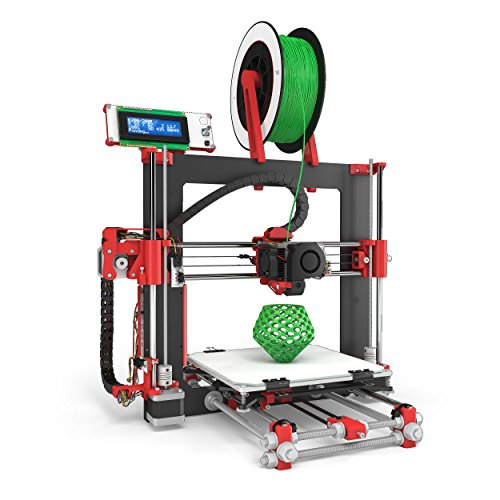
\includegraphics[width=0.49\textwidth]{./img/hephestos}
	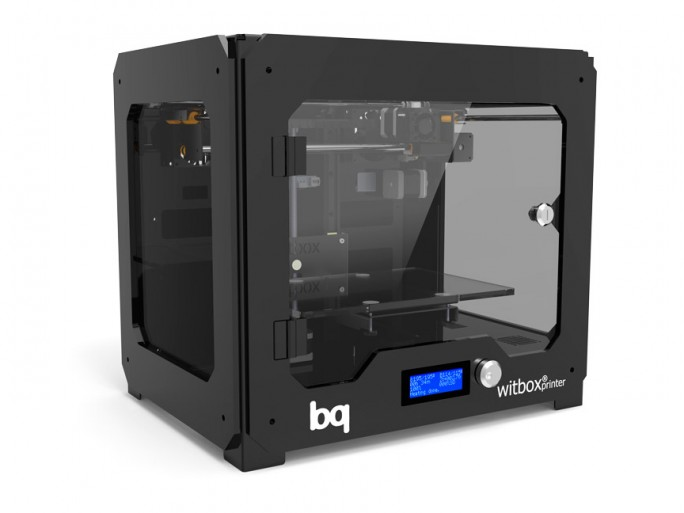
\includegraphics[width=0.49\textwidth]{./img/witbox} 
	\\(a)\hspace{7cm}(b)
	\caption{(a) Hephestos (b) Witbox} 
	\label{fig:impresoras3D}
\end{figure}

Para la fabricación del guante de PDMS se han empleado herramientas que ha simple vista pueden parecer de aplicación tan dispares como una báscula, un horno y una empalmadora de fibra (ver figura \ref{fig:herramientas}; \ref{fig:empalmadora}). La báscula utilizada es la disponible en el laboratorio de la universidad tiene ua precisión de miligramos y en este proyecto se utiliza para utilizar con exactitud la proporción del monómero y el agente de cura en la disolución de PDMS. El horno se emplea para conseguir que el PDMS se cure con la ayuda del calor en menos tiempo.

\begin{figure}[H]
	\centering
	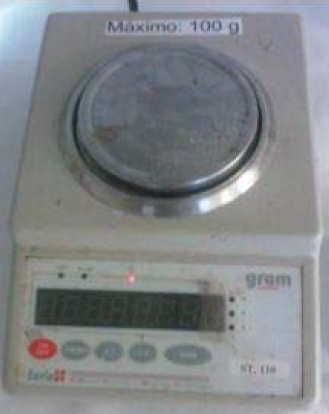
\includegraphics[width=0.3\textwidth]{./img/bascula}
	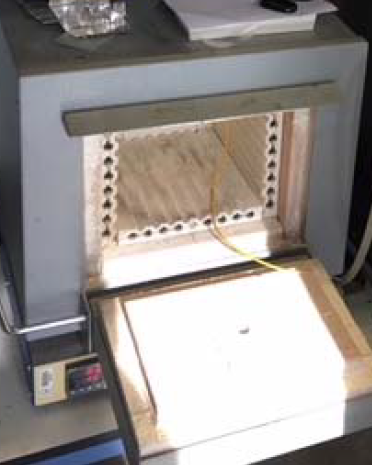
\includegraphics[width=0.3\textwidth]{./img/horno} 
	\\(a)\hspace{4cm}(b)
	\caption{(a) Báscula (b) Horno } 
	\label{fig:herramientas}
\end{figure}

Para empalmar los sensores de FBG con el resto del prototipo se emplea una empalmadora de fibra. La empalmadora utilizada tiene la ventaja de incluir un apartado para fundir los protectores termocontraibles de empalmes. 

\begin{figure}[H]
	\centering
	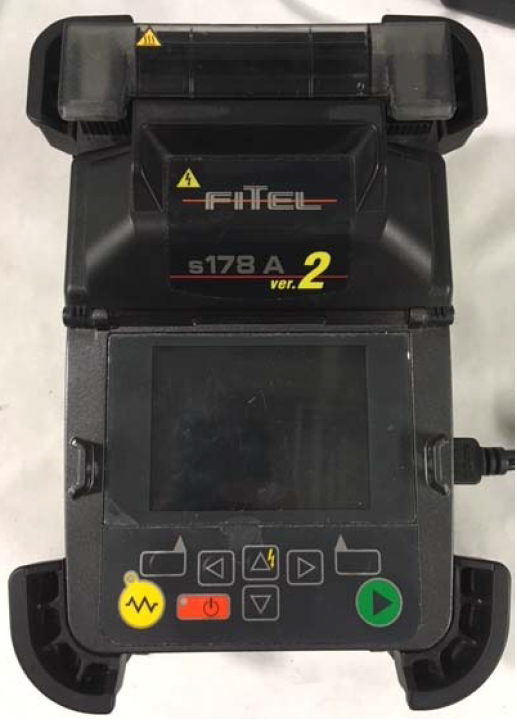
\includegraphics[width=0.3\textwidth]{./img/empalmadora}
	\caption{Empalmadora de fibra} \label{fig:empalmadora}
\end{figure}


\subsection{Proceso de fabricación del soporte físico}
\label{sec:proceso3}
%Elaboración

 \textcolor{rositaoscuro}{Elaboración/Proceso de fabricación}

Para que sea más cómoda la explicación del proceso de elaboración del prototipo se divide este en tres partes: modelado 3D, fabricación del guante y montaje del prototipo completo.

\begin{itemize}
	
% _ Modelado 3D:

	\item \textbf{Modelado 3D - Configuración 3D}
	
	Esta parte comprende el diseño del molde con el que se fabrica el guante y de la caja contenedora de todo el cableado. El software utilizado para el modelado 3D ha sido la versión de escritorio de SketchUp \cite{SketchUp}.
	
	
	Para poder producir el guante de PDMS es necesario tener un molde donde verter la disolución para darle la forma deseada. Gracias a las versatilidad de diseño que ofrece la impresión 3D se realiza con este proceso de manufactura el molde (véase figura \ref{fig:molde}). 

	\begin{figure}[H]
		\centering
		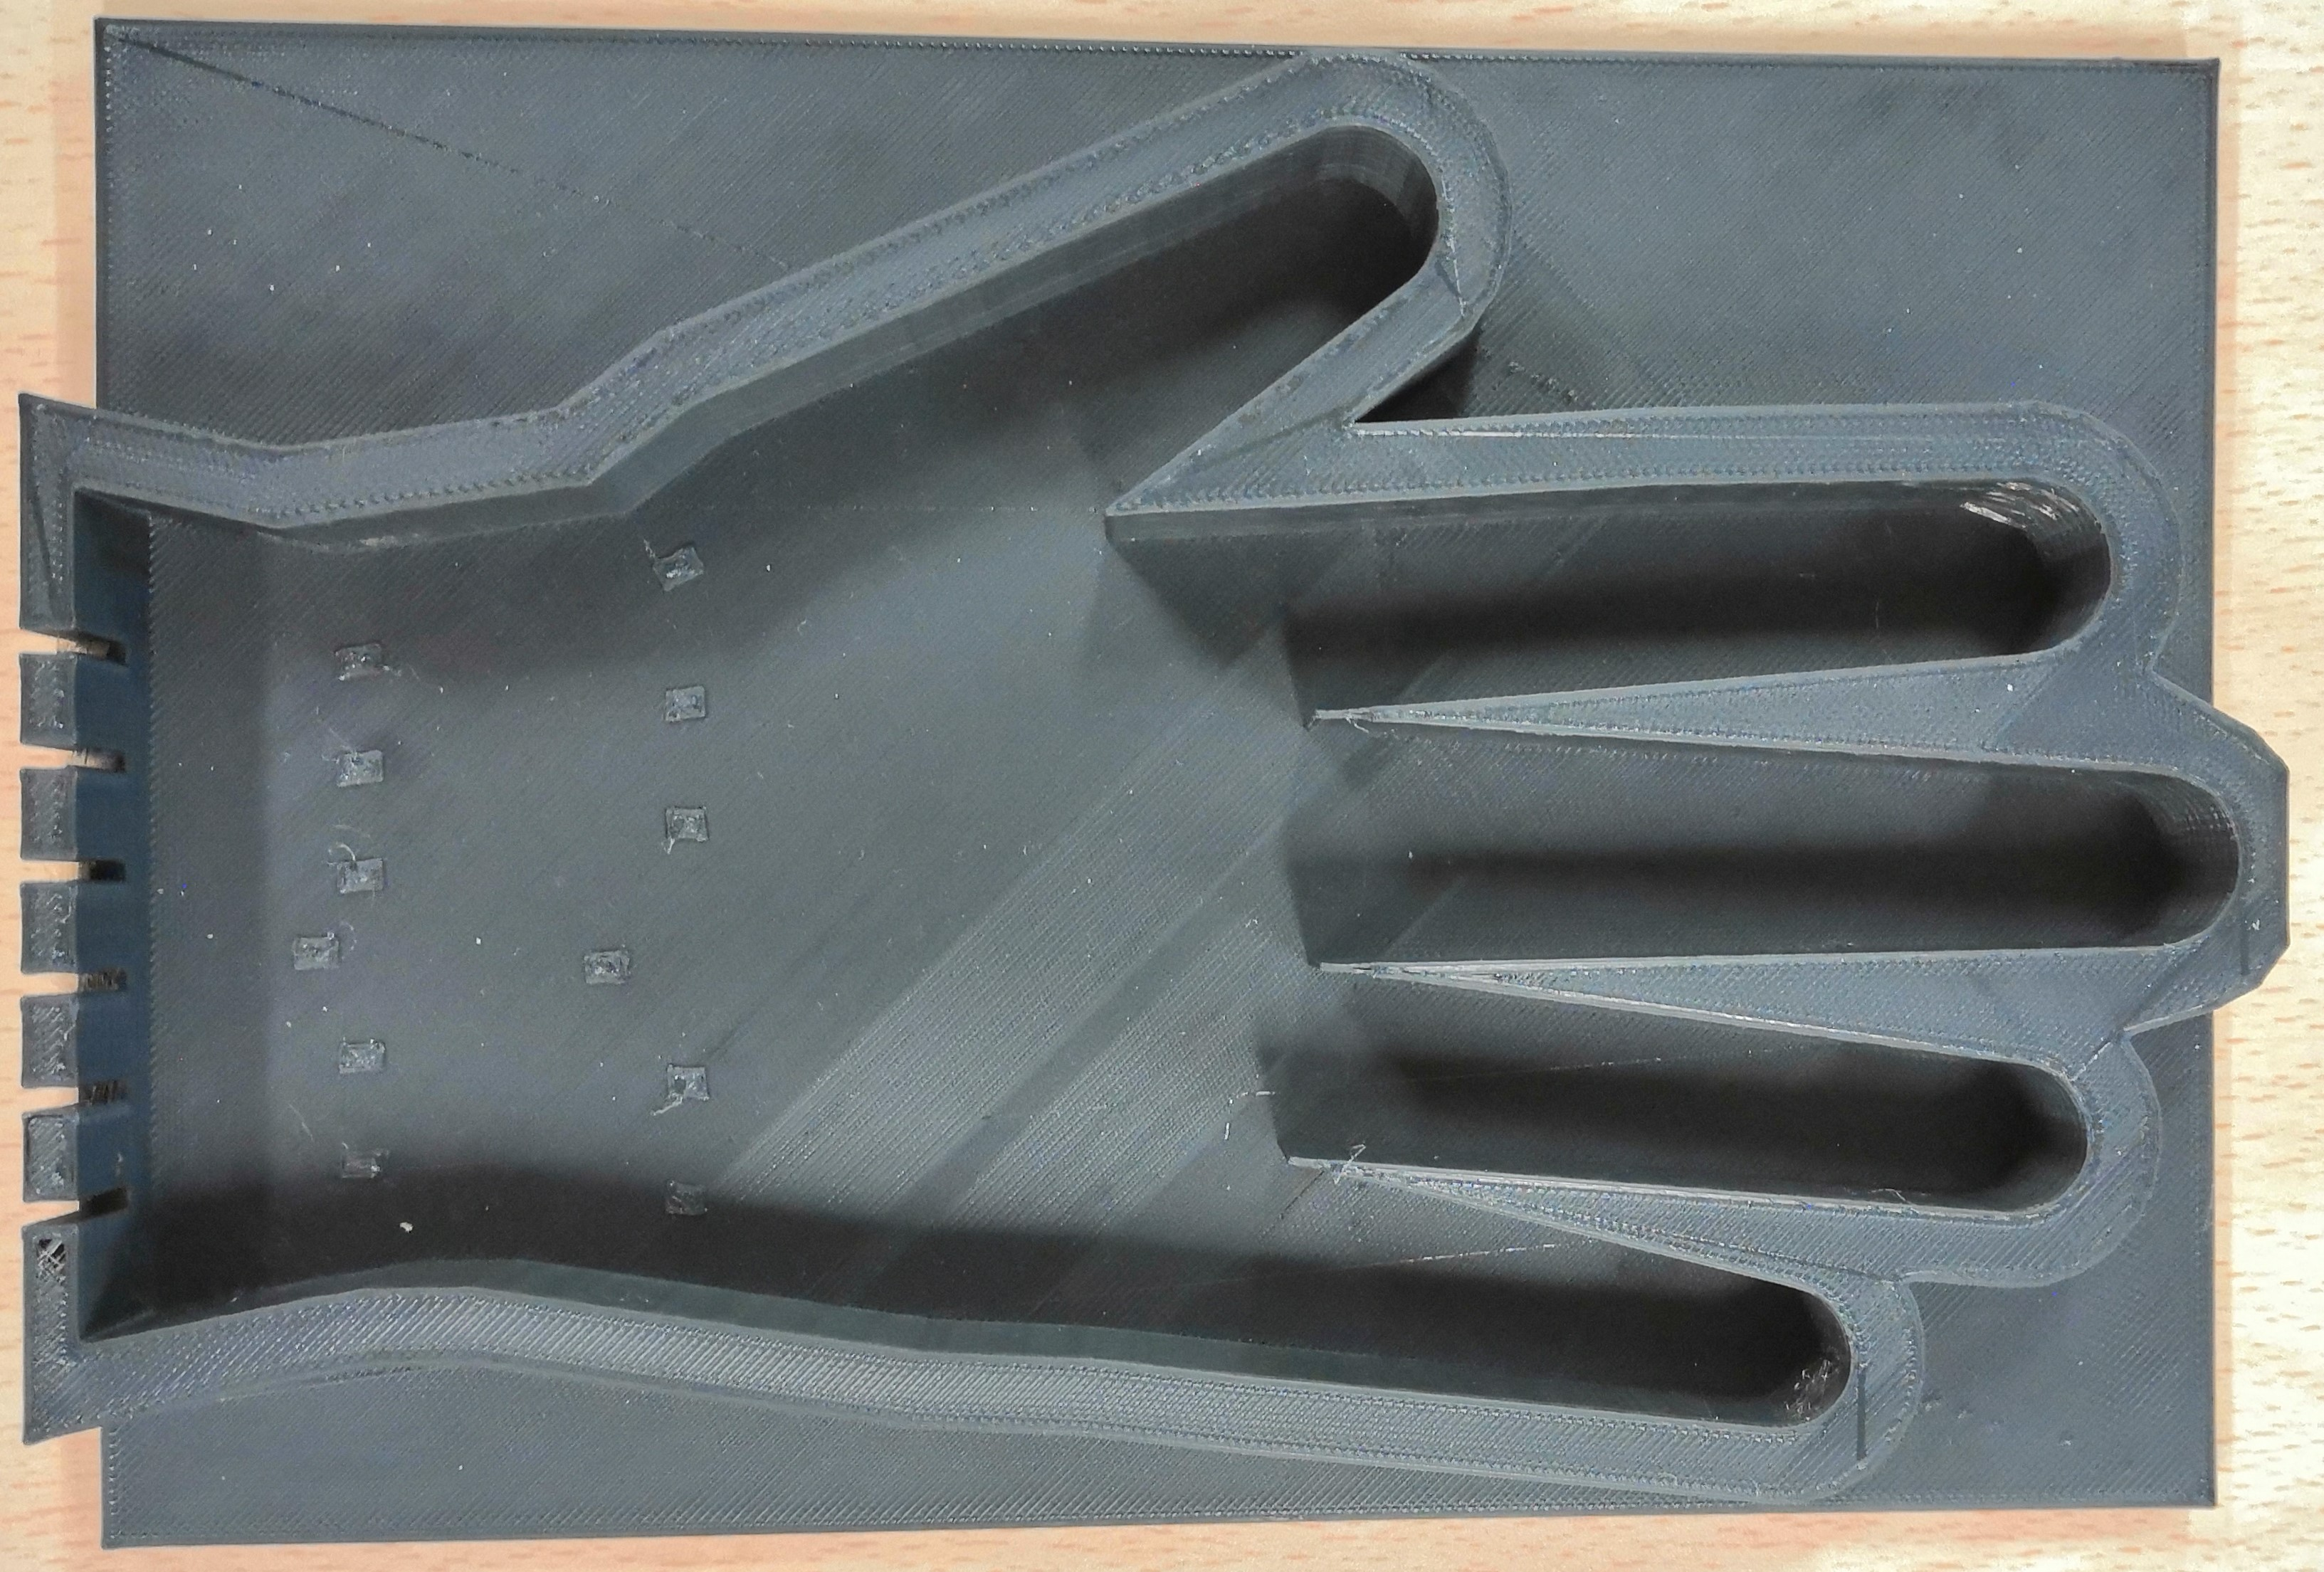
\includegraphics[width=0.6\textwidth]{./img/molde}
		\caption{Molde} \label{fig:molde}
	\end{figure}
 
 	El diseño 3D del molde se ha realizado a partir de la silueta de la huella de la mano. El recipiente con forma de mano necesita seis franjas a la altura de la muñeca para conducir por ellas las fibras de Bragg hasta el resto del prototipo. También tiene unas pequeñas muescas que sirven de guía para cuando se introduzcan la fibras en el PDMS.
 	 	
 	 	
 	En cuanto al diseño de la caja se realiza con la finalidad de contener en ella todos los cables de fibra óptica para tener un prototipo más ordenado y compacto. En la figura \ref{fig:ordenCaja} se observa la mejora que aporta el uso de esta caja, pasando de tener todas las fibras desordenadas y ocupando un espacio considerable a tenerlo todo ordenado. Además, esto protege el cableado ante roturas en traslados u otras situaciones. 
 	
	\begin{figure}[H]
	 	\centering
	 	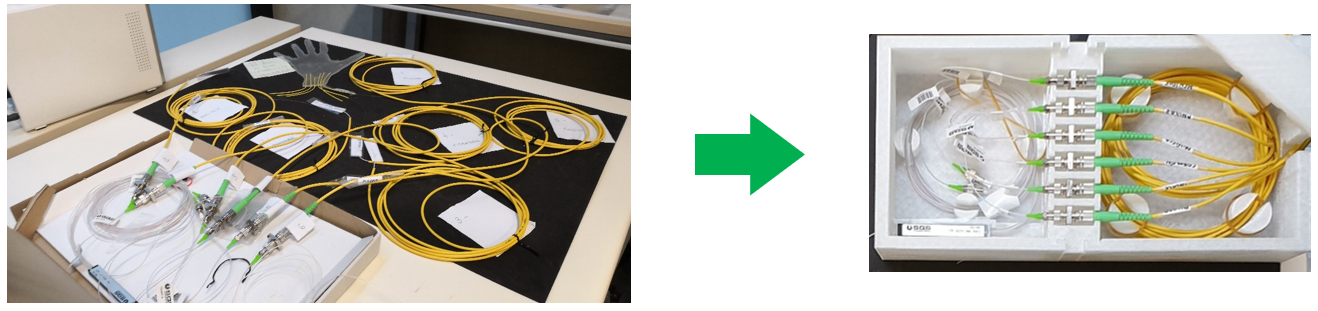
\includegraphics[width=1\textwidth]{./img/ordenCaja}
	 	\caption{Antes y después de tener la caja} \label{fig:ordenCaja}
	\end{figure}
	 	
 	El diseño se ha dividido en cuatro partes, ya que no cabía todo el diseño en las impresoras 3D disponibles. Las medidas completas son de $31.5\times15.5\times9$ cm. Tres de estas partes forman la base de la caja y una cuarta parte sirve de tapa protectora del compartimento de los conectores. La base de se divide en el compartimento para los cables de fibra procedentes del guante, el compartimento para los conectores  y el del splitter. Las cuatro partes se encajan entre ellas gracias a unas ranuras incluidas en el diseño para este fin. Todo esto se puede observar en la figura \ref{fig:caja}.
 
  	\begin{figure}[H]
		\centering
	 	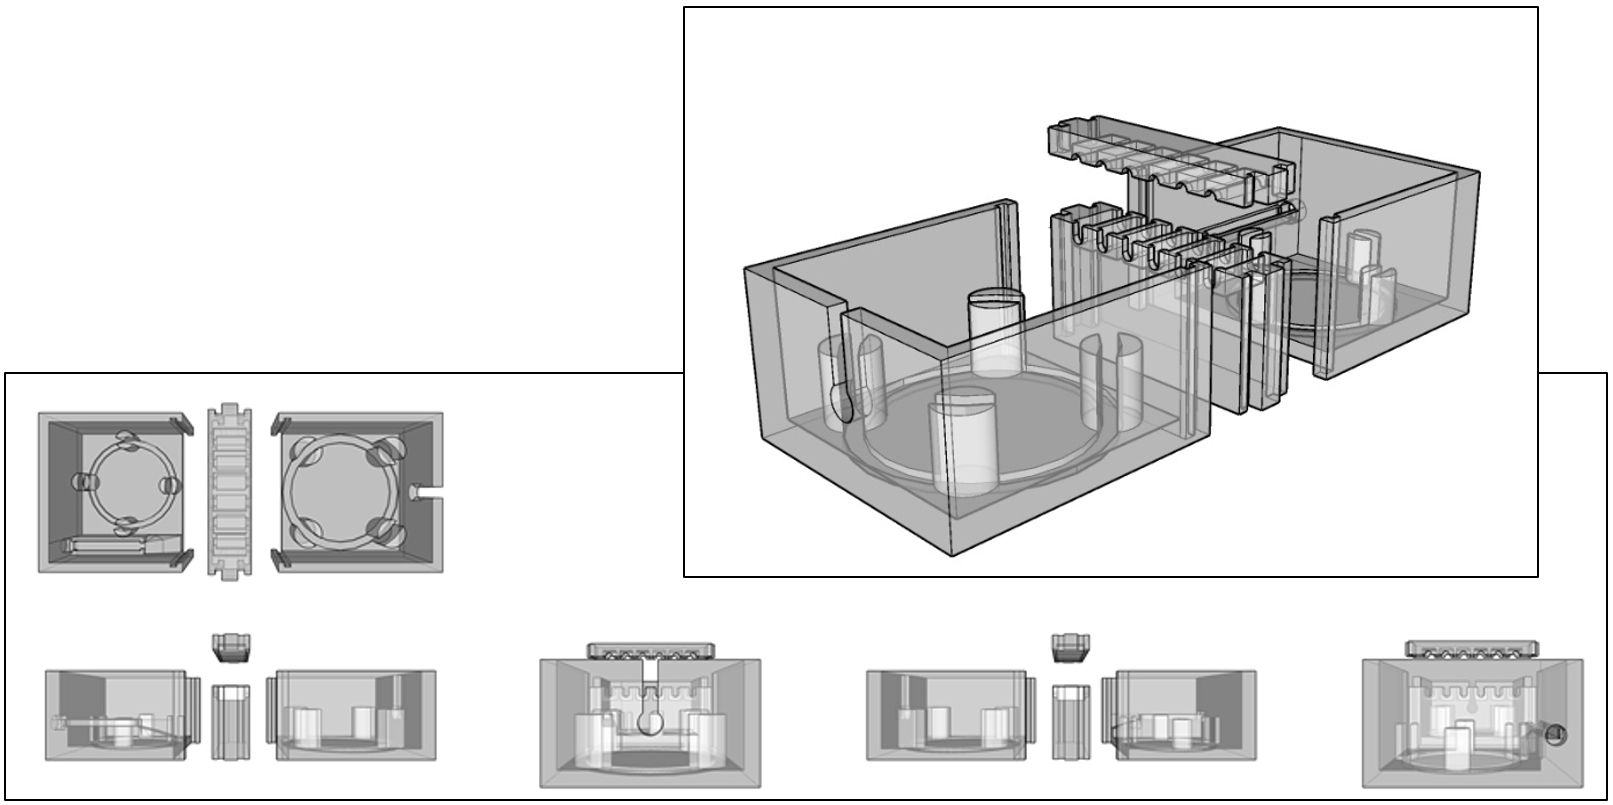
\includegraphics[width=0.8\textwidth]{./img/caja}
	 	\caption{Diseño 3D de la caja} \label{fig:caja}
	\end{figure}
 
 	Ambos diseños se imprimen en PLA por ser biodegrable. Se trata e un polímero constituido por moléculas de ácido láctico, obtenido generalmente de tratar almidón de maíz, yuca o caña de azúcar. Además tiene precio y características adecuadas para las necesidades del proyecto. \cite{bioPLA}
 	

% _ Fabricación del guante:
 
	\item \textbf{Fabricación del guante}

	Para el proceso de fabricación del guante se necesita el elastómero y el agente de cura que componen el PDMS. El PDMS utilizado corresponde a PDMS SYLGARD$^{\textregistered}$ 184 de Dow Corning (figura \ref{fig:pdms}).
			
	\begin{figure}[H]
		\centering
		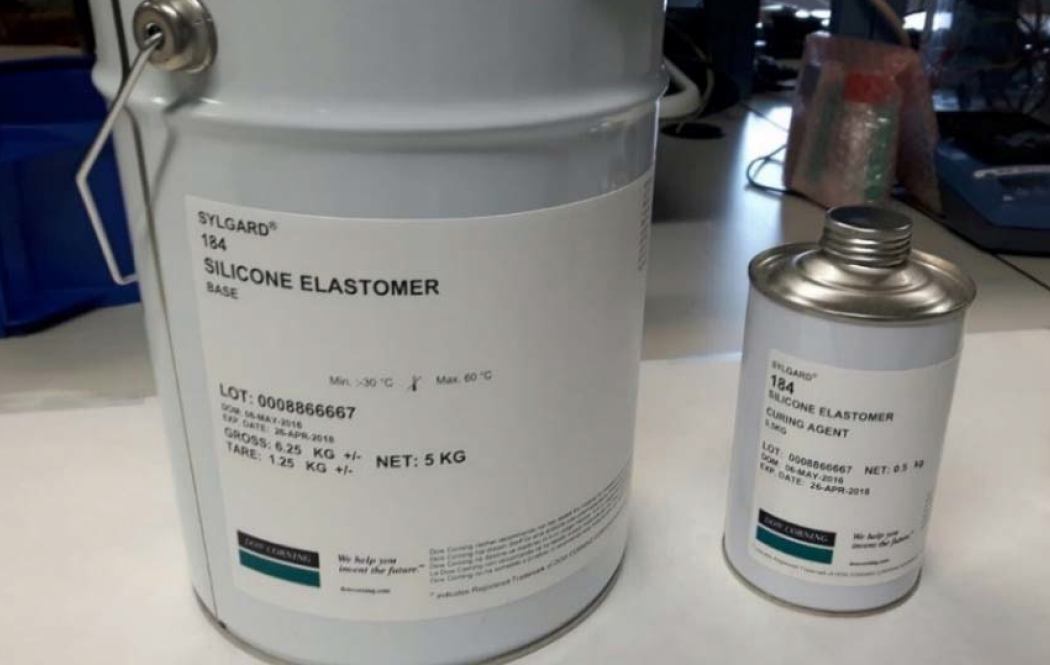
\includegraphics[width=0.5\textwidth]{./img/PDMS}
		\caption{PDMS: Elastómero y agente de cura.} \label{fig:pdms}
	\end{figure}	

	Además es necesario el molde presentado en el apartado anterior y las fibras de Bragg. En este apartado se utilizan diversas herramientas del laboratorio: capsula petri, báscula, vaso de precipitados, pipeta de plástico, espátula y  horno. 
	

	A continuación, se procede a describir por pasos el proceso de fabricación del guante:
	\begin{enumerate}
		\item \underline{Moldeado PDMS}
		
		La base de la fabricación del guante es la mezcla a realizar para la obtención de la densidad del PDMS requerida. Si se tomase una disolución muy diluida el guante no sería lo suficientemente consistente. 
		
		
		En la figura \ref{fig:fabricacionGuante} que acompaña al paso de modelado PDMS está referenciada cada foto por una letra A-D que se utiliza en el parágrafo contiguo.
		
		\begin{figure}[H]
			\centering
			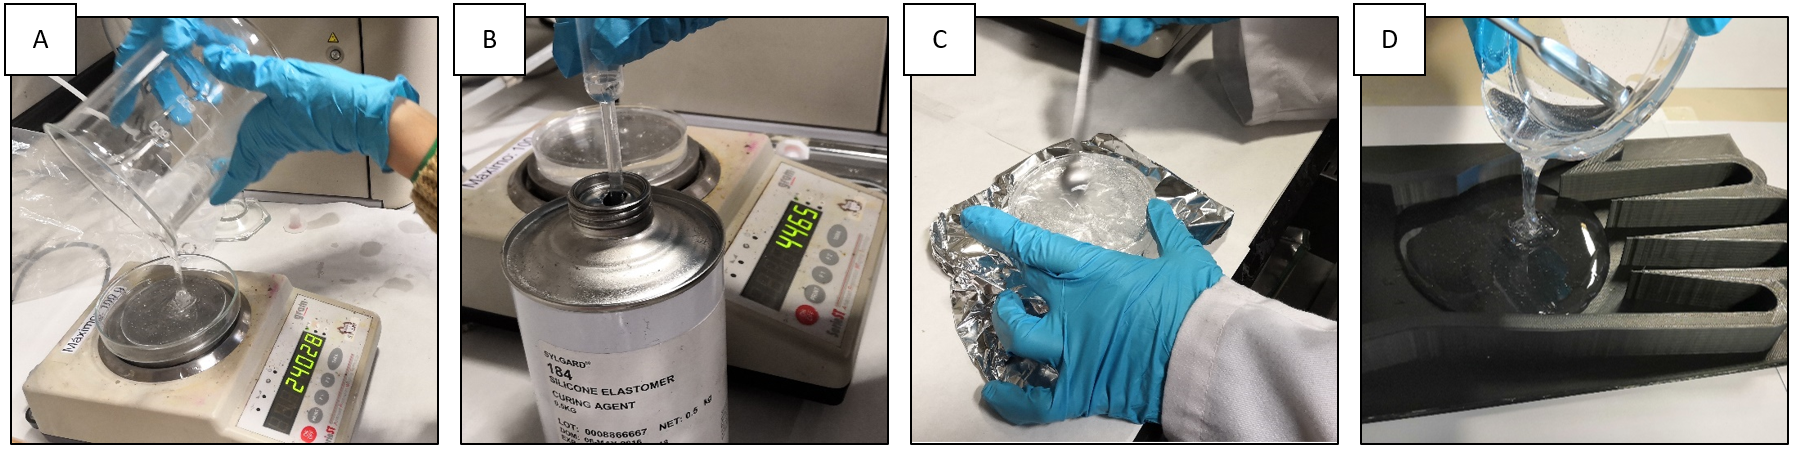
\includegraphics[width=1\textwidth]{./img/fabricacionGuante}
			\caption{Proceso de manufactura del guante.} \label{fig:fabricacionGuante}
		\end{figure}
		
		La mezcla de PDMS realiza tiene una relación agente-polímero de 1:10. Se coloca capsula petri sobre la báscula y se vierte en ella desde el vaso de precipitados 55g de elastómero [A]. Una vez se tiene la cantidad necesaria de polímero, se tabula la báscula y se toma el agente de curación desde el bote con ayuda de una pipeta de plástico [B]. Se añade al elastómero 5.5g de agente de curación. Una vez se tienen las cantidades expuestas, se mezclan durante cuatro minutos con la ayuda de la espátula [C]. Después de este paso en algunas ocasiones se generan burbujas de aire, que se pueden eliminar en un horno de vacío en pasos posteriores. En esta ocasión no ha sido necesario. Cuando se tiene una mezcla homogénea (se ha removido durante cuatro minutos correctamente) se vierte el PDMS en el molde del guante [D].  	
		
		
		Conviene recordar que tras este proceso es importante limpiar todas las herramientas utilizadas, siendo el PDMS un compuesto engorroso de limpiar. 
	
		
		\item \underline{Colocación de los sensores FBG}
		
		\begin{figure}[H]
			\centering
			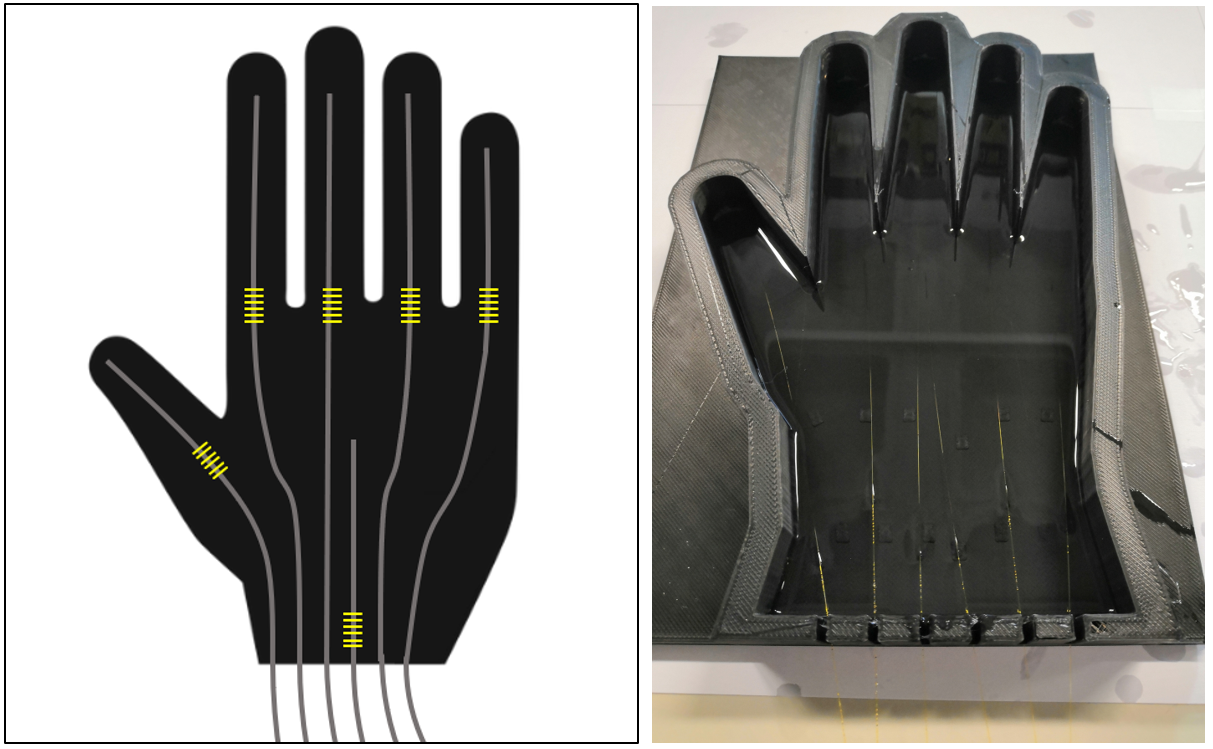
\includegraphics[width=0.65\textwidth]{./img/diagramaMano2}
			\caption{Disposición del guante sensorizado.} \label{fig:manoFBG}
		\end{figure}
		
		En este paso se colocan las fibras dentro del PDMS. En la figura \ref{fig:manoFBG} está representada la distribución de las fibras de Bragg en el PDMS frente a la colocación que se ha realizado. Aprovechando las franjas de la pared del molde y las guías de la base se han colocado las fibras dentro de la mezcla. Para que el trozo de fibra que contiene las rejillas esté en los ejes de giro de la mano (los vértices de los ángulos a medir) ha sido necesario cortar las fibras ya que el extremo superior no era necesario conectarlo posteriormente a nada. El otro extremo de la fibra se ha conducido por las franjas del molde hacia el exterior de este de manera ordenada.
		
	
		\item \underline{Curación PDMS} 
		
		Si fuera necesario quitar burbujas de aire al PDMS (como se hace refenrecia en el paso primero), sería antes de este paso cuando debería hacerse.
		
		
		Para que el PDMS se cure una opción es dejarlo al aire libre durante un par de días. Aunque es aconsejable que para que la curación sea más rápida y completa se realice en el horno. Esta afirmación se solventa en la experiencia ya que durante la realización del proyecto ha habido que dejar el PDMS curándose al aire libre, y después de tres días aún estaba el PDMS sin curar del todo. Además, cuando el PDMS estuvo curado tenía una textura más pegajosa que al utilizar el horno. Es por ello que se ha metido el molde con el PDMS y las fibras de Bragg en el horno durante cinco horas y media a $-55\,^{\circ}\mathrm{C}$). Una vez pasado ese tiempo se deja reposar una hora dentro del horno apagado. 
		
		
		\item \underline{Desmoldar}
		
		\begin{figure}[H]
			\centering
			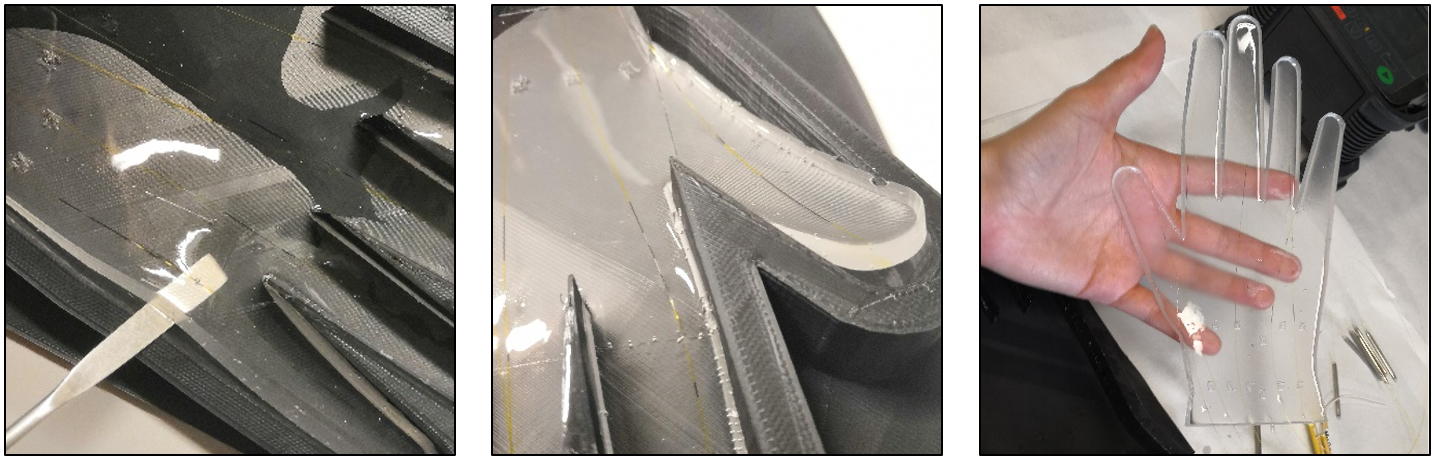
\includegraphics[width=0.75\textwidth]{./img/fabricacionGuante2}
			\caption{Desmoldado del guante.} \label{fig:fabricacionGuante2}
		\end{figure}
	
		Para finalizar el proceso de moldeado del PDMS hace falta retirar el PDMS con los sensores embebidos del molde. Este paso hay que realizarlo con mucha paciencia y cuidado. El PDMS está adherido al molde. Para ello se ha necesitado la ayuda de la espátula. En la figura \ref{fig:fabricacionGuante2} se puede representa este paso.
		

	\end{enumerate}
	
\underline{\textit{Nota:}} Cabe mencionar que durante la realización del proyecto este proceso ha sido necesario realizarse varias veces debido a los errores que han sucedido. Se detalla mejor en el apartado de resultados y conclusiones.
		

	
	
	

	
% _ Montaje completo:	
	
	\item \textbf{Montaje completo}
	
	En este punto se tiene la estructura del guante fabricada. Hace falta proceder al acoplo de este al sistema copleto.
	
	
		Además es necesario el molde presentado en el apartado anterior y las fibras de Bragg. En este apartado se utilizan diversas herramientas del laboratorio: capsula petri, báscula, vaso de precipitados, pipeta de plástico, espátula y  horno. , cortadora de precisión, alcohol, servilletas específicas para limpiar fibra, empalmadora, mechero y empalmes por fusión.
	
	
	
	-----------
	
	
	Empalmar
	
	\textcolor{rositaoscuro}{Las siguientes figuras la puedo poner por separado, en la explicacin del procesado de emapalmar.}
	\begin{figure}[H]
		\centering
		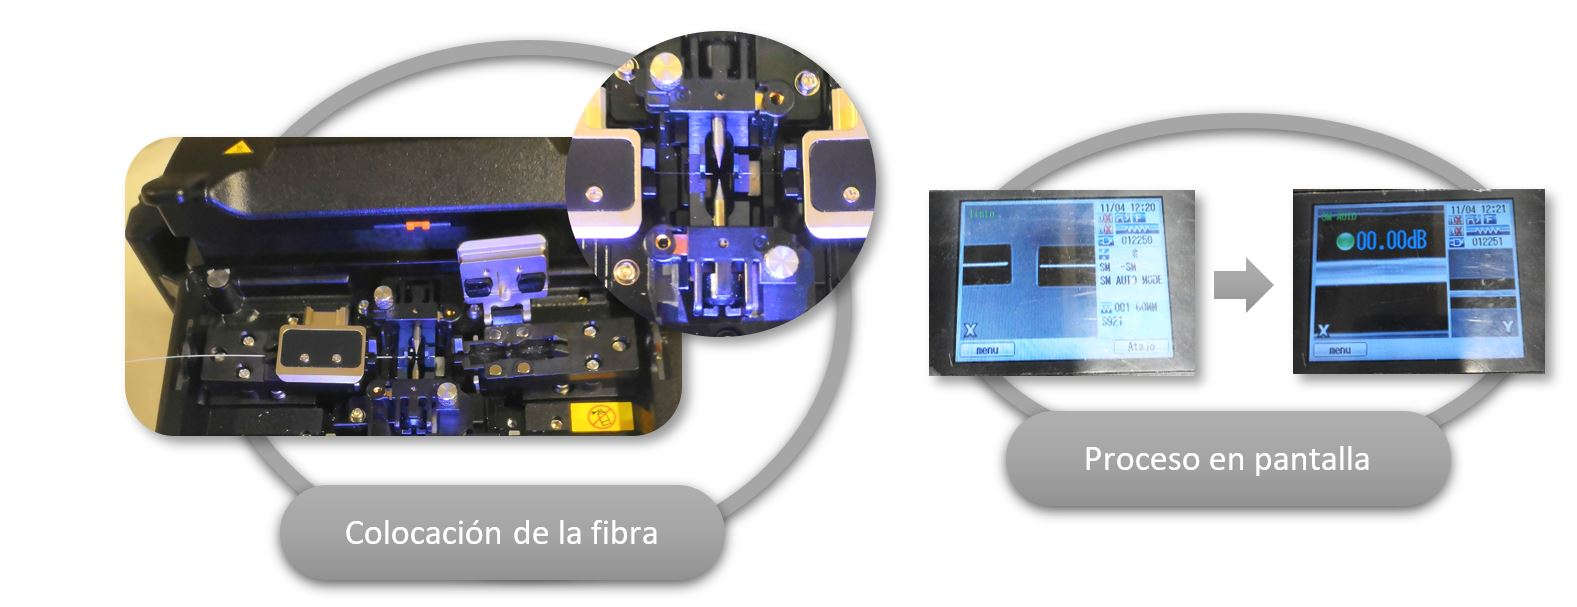
\includegraphics[width=0.95\textwidth]{./img/fusionFOpractica}
		\caption{Colocación de la fibra en la fusionadora y proceso por pantalla.} 
		\label{fig:fusionadora}
	\end{figure}  
	
	\begin{figure}[H]
		\centering
		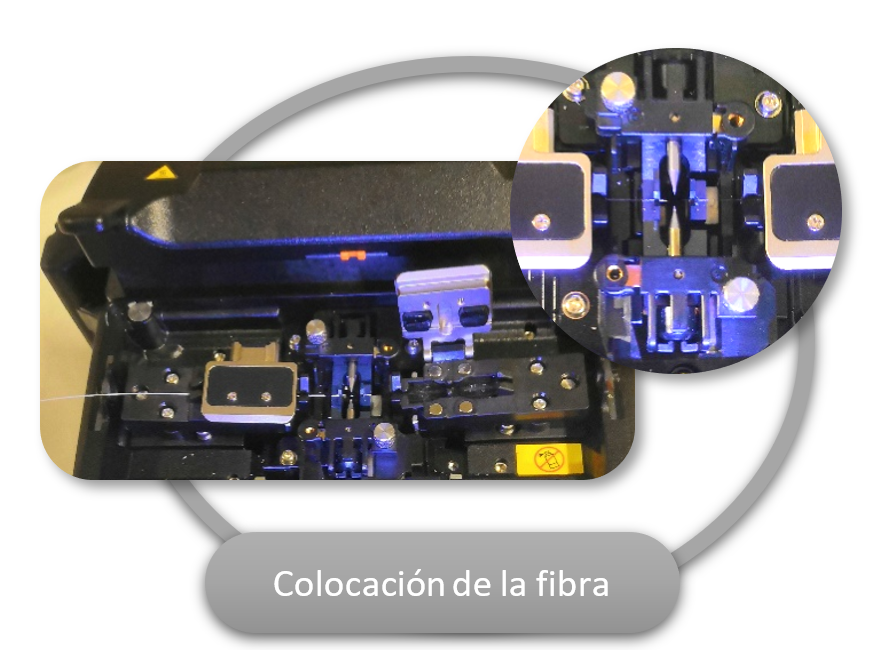
\includegraphics[width=0.6\textwidth]{./img/colocacionFibra}
		\caption{Colocación de la fibra en la fusionadora y proceso por pantalla. }
		\label{fig:colocacionFibra}
	\end{figure}  
	
	\begin{figure}[H]
		\centering
		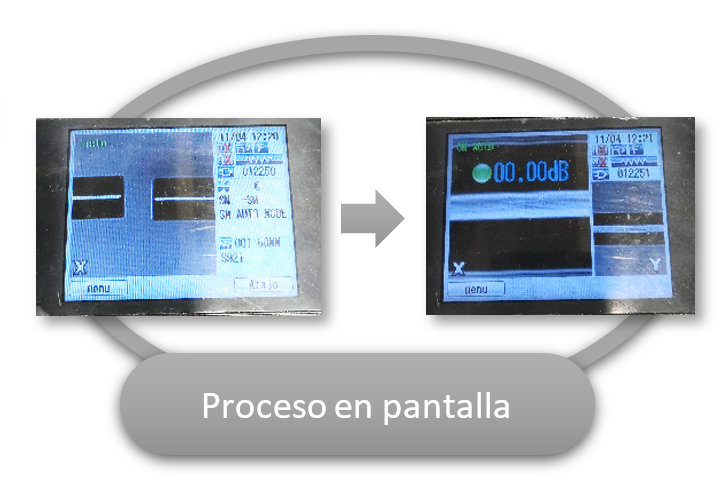
\includegraphics[width=0.5\textwidth]{./img/procesoPantalla}
		\caption{Colocación de la fibra en la fusionadora y proceso por pantalla. } 
		\label{fig:procesoPantalla}
	\end{figure}  
	
	-----------
	
	\begin{figure}[H]
		\centering
		\includegraphics[width=1\textwidth]{./img/diagramaFBG}
		\caption{Diagrama de conexiones de elementos del prototipo.} \label{fig:diagramaFBG}
	\end{figure}
	
	
	Como se representa en la figura \ref{fig:diagramaFBG}, el guante que se coloca en la mano a medir está compuesto por seis fibras de Bragg (una por cada dedo y la muñeca) embebidas en PDMS. El PDMS tiene la forma de la huella de una mano, hasta la muñeca. Desde dónde salen las seis fibras de Bragg hasta empalmarse con fibra óptica monomodo (en amarillo), estas fibras se unen mediante conectores al multiplexor (dejando dos fibras del multiplexor sin darle uso). El multiplexor va conectado a la fuente alimentada por la red eléctrica. La fuente está a su vez conectada mediante fibra óptica al interrogador, conectado al ordenador por cable eléctrico.
	
	
	
	
\end{itemize}

asdf




Para determinar la valid


\subsection{Funcionamiento}
\label{sec:funcionamiento3}
asdf

En cuanto al funcionamiento físico del prototipo la fuente  (alimentada por una red de corriente alterna, de $\sim$230V a 50Hz) el interrogador emite un pulso de luz. 



En este, en un sentido de la propagación la señal se multiplexa de una a ocho fibras y en el otro combina los pulsos de retorno de las seis fibras de FBG (dos fibras del multiplexor no se utilizan). 

Ver figura \ref{fig:diagramaFBGfuncionamiento}.

\begin{figure}[H]
	\centering
	\includegraphics[width=1\textwidth]{./img/diagramaFBGfuncionamiento}
	\caption{Diagrama de funcionamiento del prototipo.} \label{fig:diagramaFBGfuncionamiento}
\end{figure}



\begin{figure}[H]
	\centering
	\includegraphics[width=1\textwidth]{./img/interfazSM}
	\caption{Interfaz del programa de labview.}
	\label{fig:interfaz}
\end{figure}




\section{Resultados y análisis}
\label{sec:resultados3}

